%% LyX 1.6.0 created this file.  For more info, see http://www.lyx.org/.
%% Do not edit unless you really know what you are doing.
\documentclass[12pt,english]{extarticle}
\usepackage{mathptmx}
\usepackage[T1]{fontenc}
\usepackage[latin9]{inputenc}
\usepackage{geometry}
\geometry{verbose,letterpaper,tmargin=1.5cm,bmargin=1.5cm,lmargin=2.5cm,rmargin=2.5cm,headheight=1.5cm,headsep=1.5cm,footskip=1.5cm}
\setcounter{tocdepth}{2}
\setlength{\parskip}{\smallskipamount}
\setlength{\parindent}{0pt}
\usepackage{color}
\usepackage{prettyref}
\usepackage{float}
\usepackage{amsmath}
\usepackage{graphicx}
\usepackage{amssymb}


%%%%%%%%%%%%%%%%%%%%%%%%%%%%%% LyX specific LaTeX commands.
%% Because html converters don't know tabularnewline
\providecommand{\tabularnewline}{\\}

\AtBeginDocument{
  \def\labelitemiii{\(\triangleright\)}
}

\usepackage{babel}

\begin{document}

\title{\textcolor{black}{ParaTools} Manual}


\date{2011}

\maketitle
\noindent \begin{center}
Version 2.0
\par\end{center}

\pagebreak{}

\tableofcontents{}

\pagebreak{}


\part{New in Version 2}

This manual is in update process from version 1 to version 2. All
chapters, whose chapter titles are given in red color are still of
version 1 (and all their sub-chapters). All chapters with chapter
titles in black should at least be about ParaTools version 2, even
if they might not yet be completely finished. 


\section{New features}

It is now possible to introduce a user defined coordinate description
of any kind, as long as it fulfills some requirements. This works
only with direct function call of the routines.

New routines for finding transition states have been included: they
are eigenmode routines of dimer and Lanczos type.

New routines for interpreting path searching output further.


\section{Change in the routines}

All routines can now be accessed via the general command {}``paratools''
making it obsolent to have tools directory with many separate files
in PATH set.

Attention: some of the additional routines have been different names
in the command line, which should be more convinient. The direct usage
of the tools from subdirectory is also still possible but it is recommended
to use them all via the command line to reduce the complete number
of available routines.

Some of the parameternames in path searcher have been adapted. 

The storing of reusable results in path searcher is now handled differently,
parameters about it have to be adapted and renamed.

The final path in path searching routines is now also provided in
user readable files.

The routine path2plot can now also extract force and energy information
from the path.pickle files and interpolate/plot them.

Several routines, which required explicitely a path.pickle as input,
can now read in their informations in user readable way.


\part{General Overview}

The goal of the Toolbox ParaTools is to provide functionalities to
a number of different quantum chemistry calculators. The functionalities,
working on the geometries of a given molecular object, should cover
a wide range of different features wanted with a focus on methods
helping to search transition states. The quantum chemistry calculators,
VASP or ParaGauss, are used as a kind of black box, which should deliver
forces and energies to the toolbox after getting to know the geometry
they should work on. In this way all calculators should be usable
with every tool. In cases where there are several geometries known
at the same time, the toolbox allows to calculate at least some of
them in parallel. 

ParaTools uses another toolbox the Atomic Simulation Environment (ASE)
as a basis, thus all the ASE functionalities are in principle available,
while ParaTools takes advantages of the description of atoms objects
and especially the wide range of quantum chemistry calculator wrappers.
This manual will only talk about the already tested quantum chemistry
calculators VASP and ParaGauss. If there is a want for another one,
the most recent version of the ASE manual will tell about their usage. 

All the code for the toolbox is written in python, thus flexible to
use and easy to adapt.

Chapter \ref{sec:What-Is-in} gives a short motivation for using ParaTools. 

In chapter \ref{sec:How-to-Find} a way of trying to find an approximated
transition state, as a good starting point for a local transition
state search is described. This is one of the best explored feature
of ParaTools. There are many tools which help to find the best approximation
there. There is a short introduction to how to use them.

More details about all the functions of ParaTools and some of the
ASE framework can be found in part \ref{par:Toolbox functions}. 

Part \ref{par:Setting-up-the} and \ref{par:Parallel-Calculations}
are about the way to set up the system in order to make the toolbox
run. Part \ref{par:Parallel-Calculations} describes how calculations
can be done in parallel. 

\pagebreak{}


\section{Short Motivation for Using ParaTools\label{sec:What-Is-in}}

%
\begin{figure}[H]
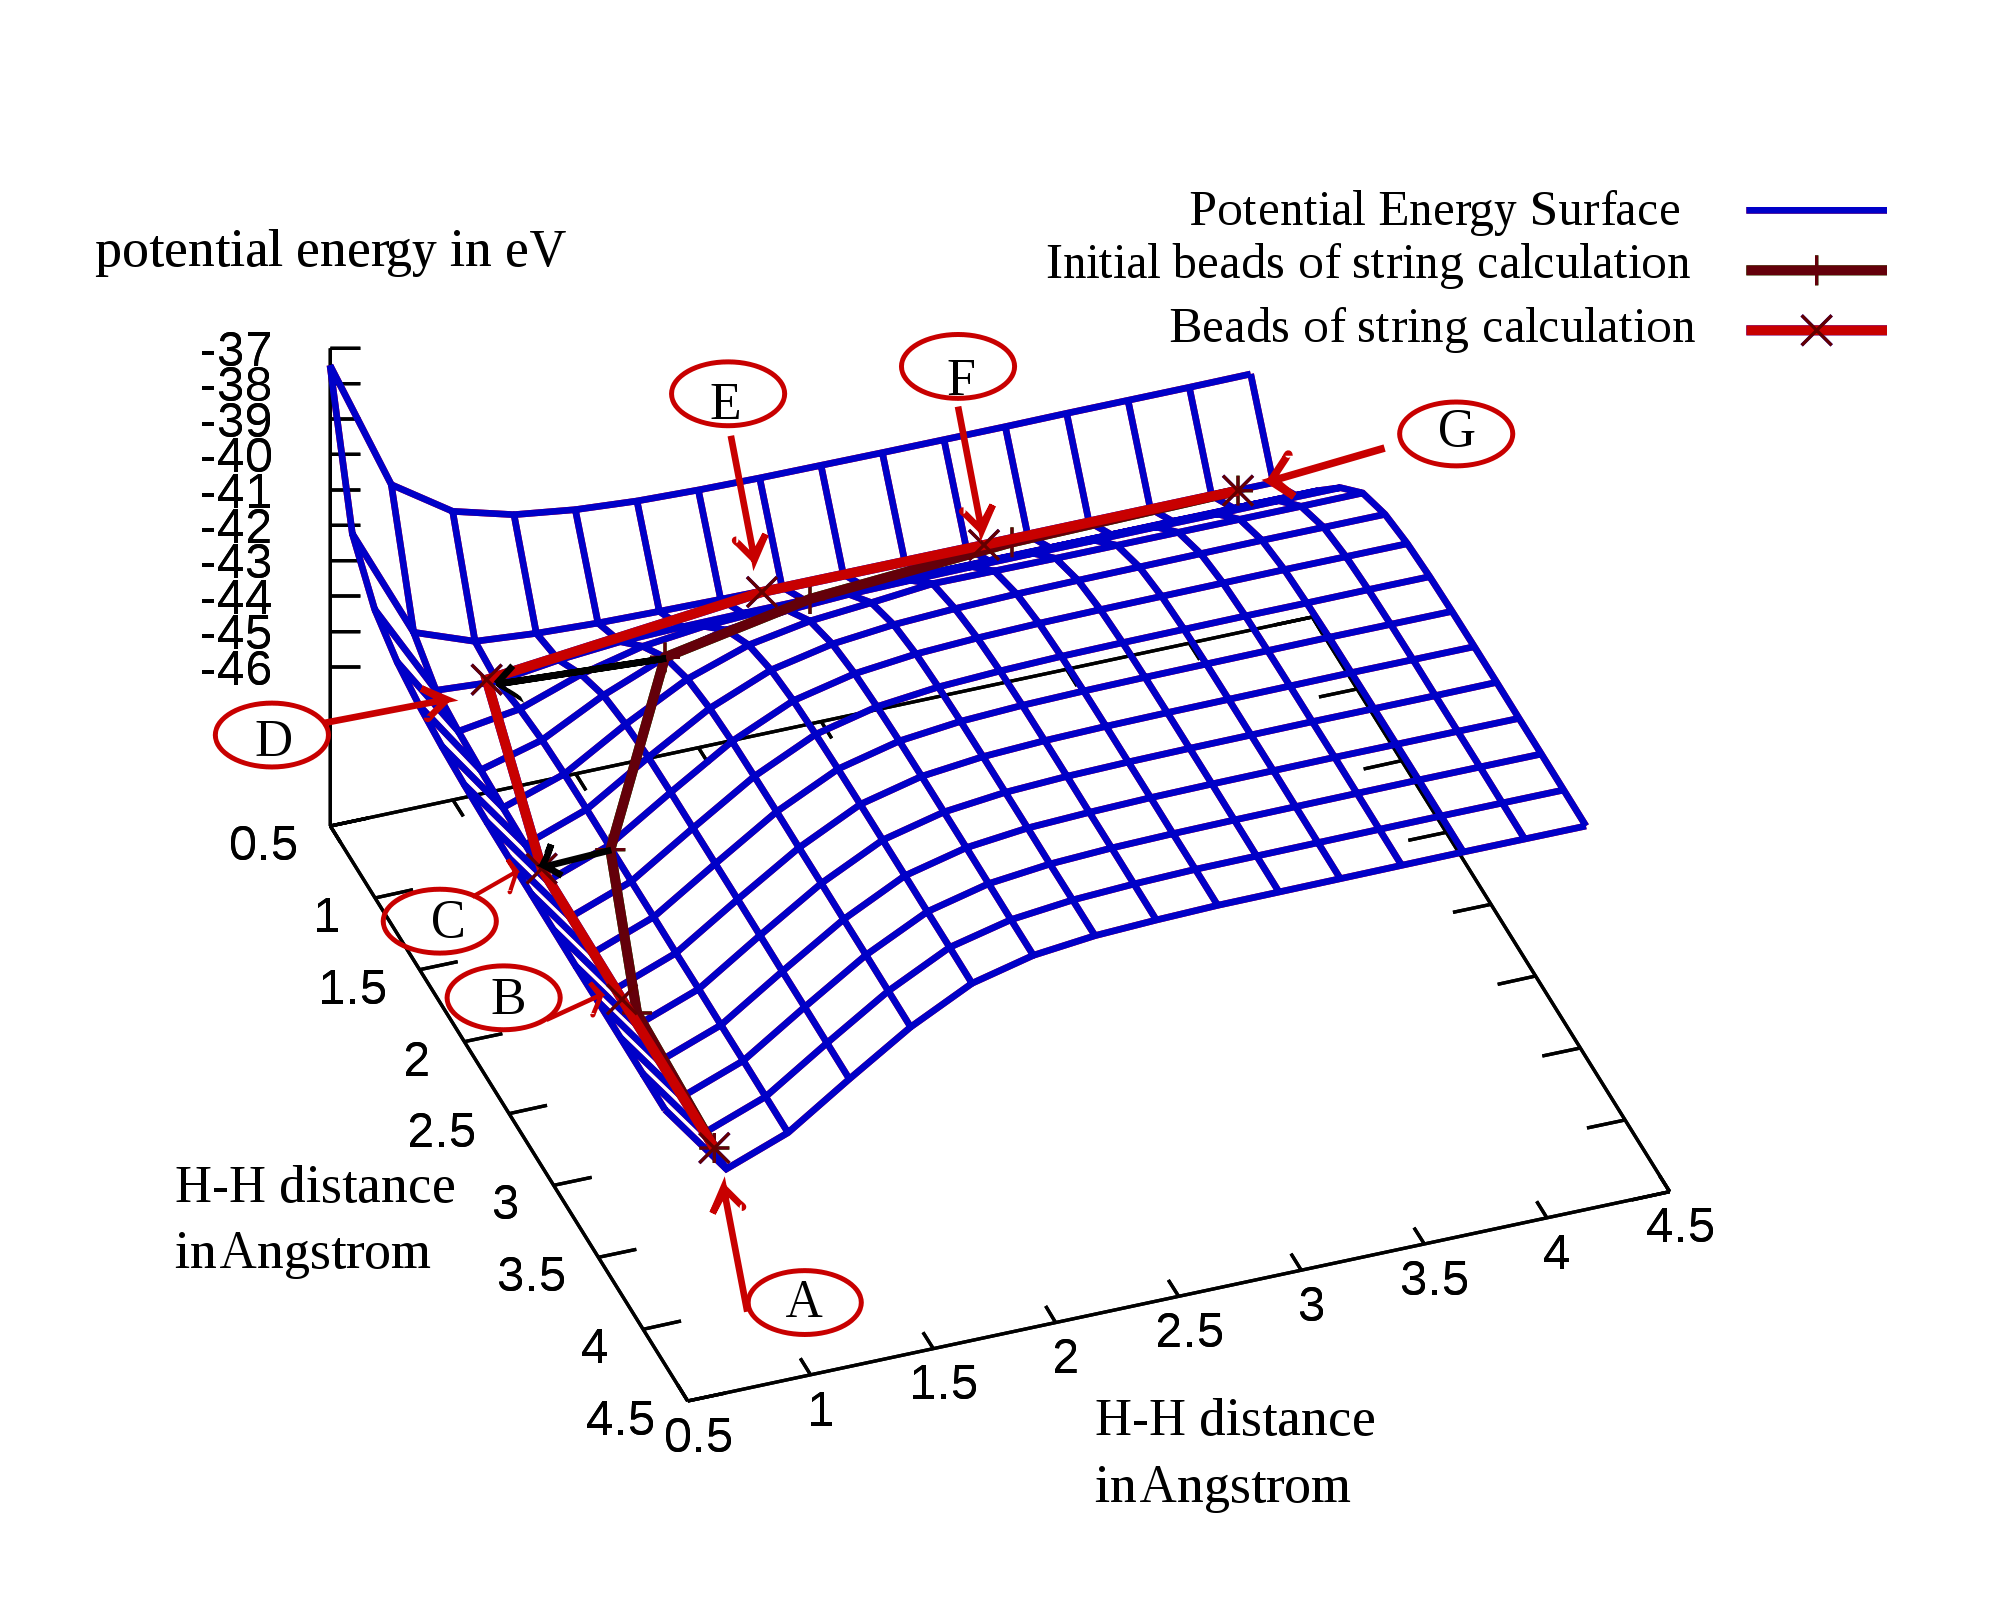
\includegraphics[scale=0.3]{Pictures/h3surfaceandstrings2}

\caption{\textbf{Possible tasks on a potential energy surface: relaxing the
brown initial path to the read one, which is much nearer the expected
reaction path, finding the best approximation for a transition state
(here point D) on the path. Or calculating the frequencies (not shown)
for the points. And of course having the complete potential energy
surface at least in a specified range. On a surface of three linear
H-atoms all this is rather easy but in general one would not be able
to calculate the energy surface to such accuracy. Then the tools of
ParaTools will provide a great help for at least the first tasks.
(All the shown calculations for the picture were done with help of
ParaTools)}}

\end{figure}


\pagebreak{}


\section{Usage}

First one has to set the environment variable PYTHONPATH to give python
the chance to find the code. PYTHONPATH should contain the path to
the sources of both ASE and ParaTools. On our local cluster this can
be just: /users/alexei/PYTHON. So for a bash shell one has to do:

\textit{export PYTHONPATH=/users/alexei/PYTHON:\$\{PYTHONPATH\}}

or for a tcsh shell:

\textit{setenv PYTHONPATH /users/alexei/PYTHON:\$\{PYTHONPATH\}}

To find the programs directly one has to include the paths to the
PATH variable:

\textit{/users/alexei/PYTHON/pts/bin/ }and\textit{ users/alexei/PYTHON/pts/tools/.}

Now one can run already the first commands. But be aware that most
of the quantum chemistry calculators need also some more specific
environment variables to make them run correctly.

For Vasp for example: 

\textit{VASP\_PP\_PATH=/users/alexei/devel/vasp/ase-vasp/mypps}

and

\textit{VASP\_COMMAND=\textquotedbl{}qrsh -cwd -pe \textbackslash{}{*}
2 -now no -N v-single\_point mpirun /users/alexei/bin/vasp\textquotedbl{}}

(the last one will make all actual VASP calculations run on separate
processes scheduled from the python program on its own)

All the functionalities of ParaTools can be used both interactively
and direct in a small python program. For the first way they are collected
in the central command. These command is situated in \textit{\$PYTHONPATH/pts/bin/}
and is called paratools. The usage is the following:

\textit{paratools CMD {[}--help| ...]}

CMD is the specification what one wants to calculate thus for example
string, forces or frequencies. With the option --help one would get
a description on how the special command works and which options one
could or has to set.

So for example to run now a program one needs geometry input file(s)
for example in xyz (jmol) format or vasp POSCAR style. Addtional one
needs a file containing the settings about the wanted calculator (say
for example calc.py) containing;

\textit{calculator = <Calculator Name> (<settings>)}

So for example:

\textit{calculator = Vasp(ismear = 0, ispin = 2)}

To run now a calculation searching for a minimum enery path do:

\textit{paratools string \nobreakdash-\nobreakdash-calculator <calculator
file> <minimum 1> <minimum 2>}

or

\textit{paratools neb \nobreakdash-\nobreakdash-calculator <calculator
file> <minimum 1> <minimum 2>}

Consider that the two minimum beads of the string will not move and
thus should be already converged minima.

For only checking on the energy or the forces of a geometry do:

\textit{paratools energy \nobreakdash-\nobreakdash-calculator <calculator
file> <minimum 1>}

\textit{paratools forces \nobreakdash-\nobreakdash-calculator <calculator
file> <minimum 1>}

There are many other tools of which quite a lot is about helping to
interprete the output of paratools pathsearcher routines or visualize
parts of it. They might require the output of a preceeding neb or
string calculation. But others are independant of it or allow another
kind of usage. To see a list of all available commands for paratools
call

\textit{paratools --help}

Here one can find for example the tool ts\_and\_mods, for which the
simplest kind of usage looks like: 

\textit{paratools ts\_and\_mods <path.picke file>} 

\pagebreak{}


\section{How to Find a Transition State (With Help of ParaTools)\label{sec:How-to-Find}}

This is the somewhat central feature of the toolbox. After initialization
of ParaTools (as described in part \ref{par:Setting-up-the}) \textcolor{black}{it
}is ready to start. 
\begin{itemize}
\item The required setting should be changing some environment variables,
thus for a batch shell:


\textit{export PYTHONPATH=/users/alexei/PYTHON:\$\{PYTHONPATH\}}

\textit{export PATH=/users/alexei/PYTHON/pts/bin/:\$\{PATH\}}

\textit{export VASP\_PP\_PATH=/users/alexei/devel/vasp/ase-vasp/mypps}

\textit{export VASP\_COMMAND=\textquotedbl{}qrsh -cwd -pe \textbackslash{}{*}
2 -now no -N v-single\_point mpirun /users/alexei/bin/vasp\textquotedbl{}}

\item or for a tscp shell:


\textit{setenv PYTHONPATH /users/alexei/PYTHON:\$\{PYTHONPATH\}}

\textit{setenv PATH /users/alexei/PYTHON/pts/bin/:\$\{PATH\}}

\textit{setenv VASP\_PP\_PATH /users/alexei/devel/vasp/ase-vasp/mypps}

\textit{setenv VASP\_COMMAND \textquotedbl{}qrsh -cwd -pe \textbackslash{}{*}
2 -now no -N v-single\_point mpirun /users/alexei/bin/vasp\textquotedbl{}}

\end{itemize}
%
\begin{figure}[H]
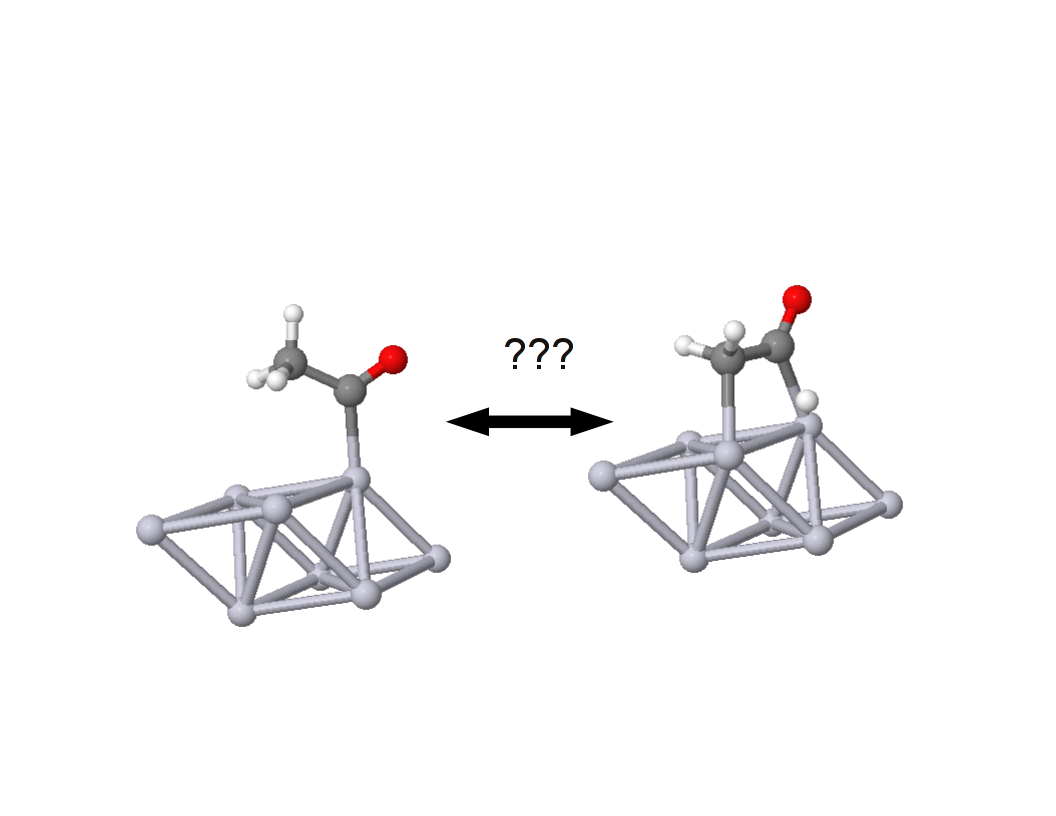
\includegraphics[scale=0.5]{Pictures/ethanoxid_question}

\caption{\textbf{Example reaction: dehydrogenation of acetyl on a Platinum
surface (111). There are two minima, calculated with fixed surface.
The search is now for the transition state between these two minima.
}\label{fig:Example-reaction:-dehydrogenation}}

\end{figure}

\begin{itemize}
\item Suppose now that there would be two minima geometries as a starting
point (Figure \ref{fig:Example-reaction:-dehydrogenation}) for which
the transition state is wanted. In this example the calculation had
been performed with VASP in an appropriate unit cell. The two minima
will be called in further steps POSCAR.left and POSCAR.right. They
are in POSCAR format, where the comment line is filled with the names
of the atoms involved. This format is easy to handle for the toolbox.
Others, like xyz formats, can be also used. But they would require
additional input for the cell, which is needed by VASP. The POSCARs
already contain the cell in a way, that the toolbox can understand.
VASP POSCARs can also contain informations about the fixing of some
(Cartesian) coordinates, if selective dynamics is set. The toolbox
can also understand this, at least as long as all the calculations
with the toolbox are performed in Cartesian coordinates. Thus in our
example, where this option is used, the surface will be fixed all
the time, when the geometry is changed.
\item The toolbox should also use the same VASP settings for calculating
the transition state. For this a small input file (figure \ref{fig:Example-file-for})
can do the job. This file may be named vasp.py for example. More about
calculators can be found in chapter \ref{sub:The-calculators}.
\end{itemize}
%
\begin{figure}[H]
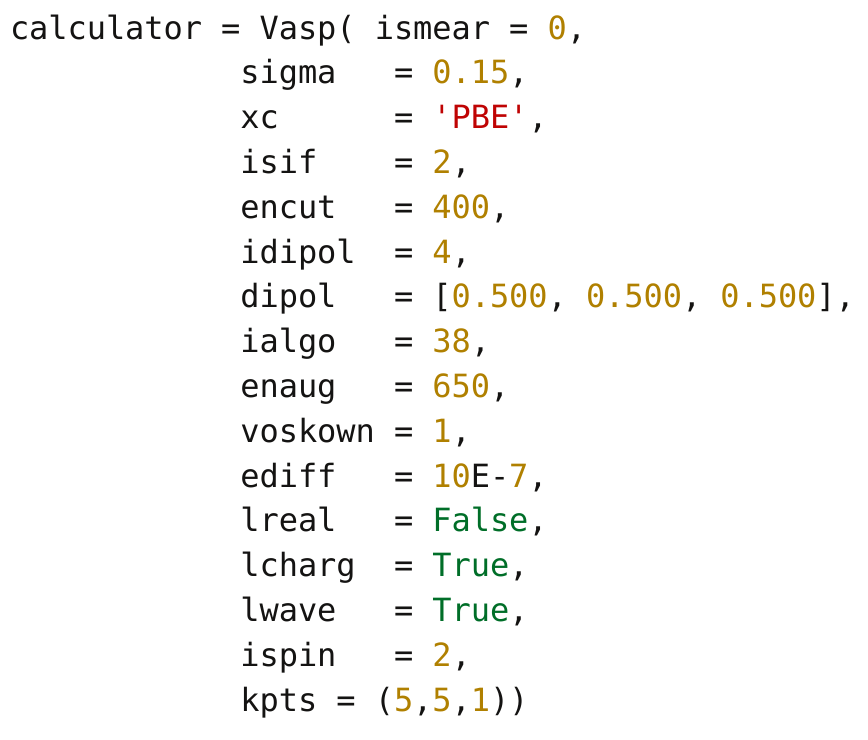
\includegraphics[scale=0.4]{Pictures/Calculator_new}

\caption{\textbf{Example file containing a VASP calculator. Most of the variables
which were specified here are common VASP variables, which are normally
given in the VASP INCAR file. Note the appearance of the kpts (k-points)
which are normally specified in a separte file. }\label{fig:Example-file-for}}

\end{figure}

\begin{itemize}
\item First step would be to verify, if the minima are really at very low
forces (this may be skipped with a high enough trust in the minimization
routines and in the transformation of the VASP specifications to the
ASE format. This can be done with a tool to calculate single point
energies or forces, found in \ref{sub:Single-Point-Energy}. 


\textit{paratools forces \nobreakdash-\nobreakdash-calculator vasp.py
POSCAR.left POSCAR.right}

This will do a single point calculation of the two minima, giving
back only the forces found there.

\item Next is to find an initial path. The main calculation will work only
with the two minima. But if already the initial path is completely
nonsense, the rest will hardly get better. For example VASP makes
use of the periodicity and one can find atoms shifted to the next
cell. Thus it is highly recommended to test the initial path the pathsearcher
would use. The tool make\_path (chapter \ref{sub:Makepath.py}) calculates
only the geometries, and thus is rather quick. As output it gives
(in xyz format) the geometries of all the beads on a possible path.
The output may be redirected from the standard output. This can be
done by:


\textit{paratools make\_path \nobreakdash-\nobreakdash-num 7 POSCAR.left
POSCAR.right > initpath.xyz}

The file initpath.xyz can now be visualized for example with jmol.
In our case this will give figure \ref{fig:Path-of-linear}.

After some rearranging of the right geometry file, the initial path
may look something like figure \ref{fig:Inital-path.}. That is much
better. 

\end{itemize}
%
\begin{figure}[H]
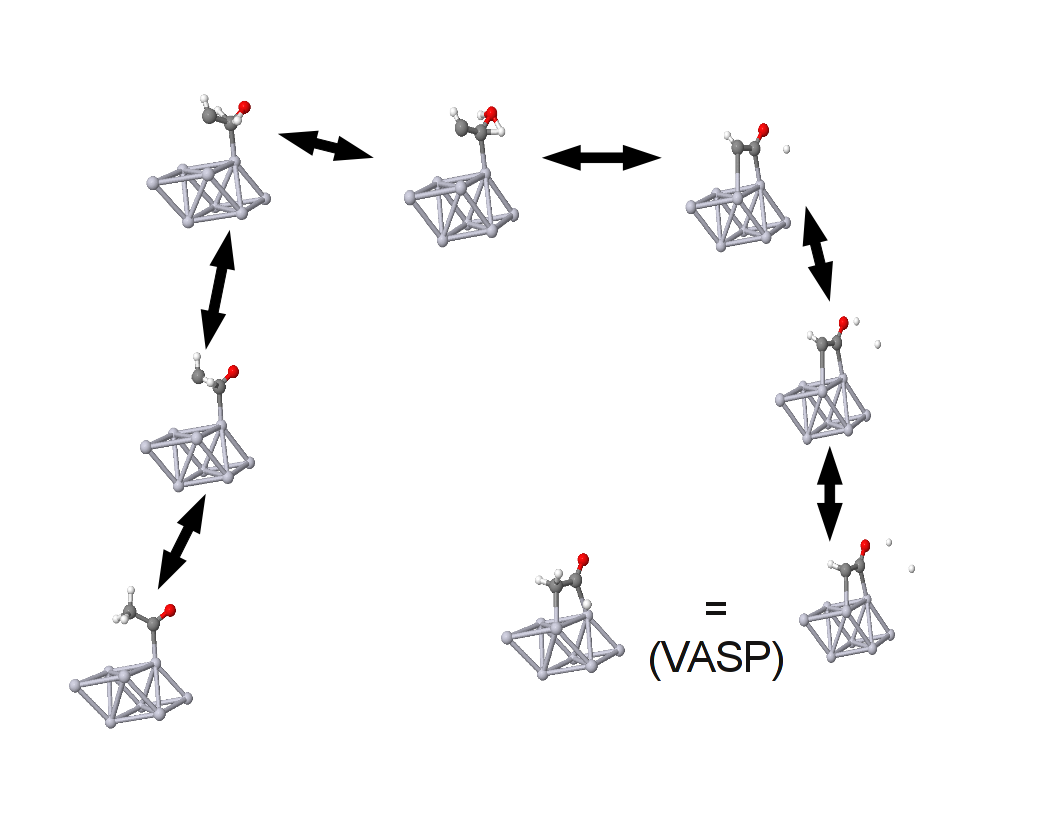
\includegraphics[scale=0.7]{Pictures/eo_wrongpath}

\caption{\textbf{Path of linear interpolation between two minima. For VASP
the two geometries at the right bottom are the same. But they make
a big difference in interpolation, as the interpolation tool does
not know anything about periodicity of the system. If the two minima
would be given as an input, the pathsearcher tool would certainly
fail to converge the resulting path. }\label{fig:Path-of-linear}}

\end{figure}


%
\begin{figure}[H]
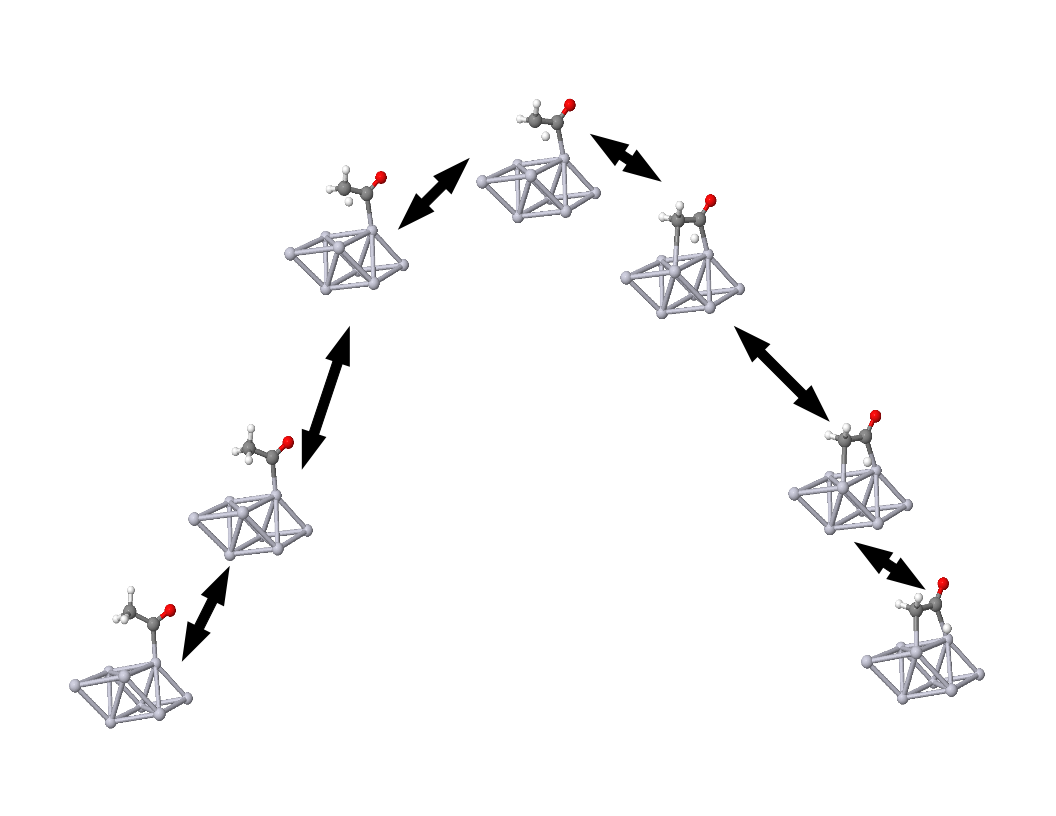
\includegraphics[scale=0.65]{Pictures/eo_initpath}

\caption{\textbf{Initial path of linear interpolation. Here the interpolation
is done between the two minima carfully avoiding to have atoms shift
the cells between them. }\label{fig:Inital-path.}}

\end{figure}

\begin{itemize}
\item The something like central routine of the toolbox is the routine which
searches the minimum energy path. It is possible to choose different
methods of it, like NEB or several string methods. This example restricts
itself to a simple string method. More about the methods and there
variants can be found in chapter \ref{sec:The-Path-Searching}.


\textit{paratools string \nobreakdash-\nobreakdash-calculator calc.py
POSCAR.left POSCAR.right}

The chapter mentioned above shows also all the parameter, which may
be chosen additionally. This tool will have to do many calculations
with the quantum chemistry program. There are several geometries (of
all the beads) known at the same time. Thus it makes sense to consider
a parallel calculations of them. How parallel calculations are done
and what is special about the serial ones is described in part \ref{par:Parallel-Calculations}.
Especially as most quantum chemistry programs have only a limited
scalability to large processor numbers having several instances of
them run at the same time with fewer processor numbers each is often
much more effective than doing all the calculations serial with the
sum of all the processors. 

\item This calculation may finished because it hit the maximum iteration,
rather than because it converged. The convergence criteria will have
been chosen too high. Still one can try to extract the best of the
results. For the last path there are some geometry files present,
called BEAD\_n and at least one approximation for the transition state
TSESTIMATE\_1, together with the corresponding MODEVEC\_1. More about
the output of the pathsearcher calculations can be found in \ref{sub:Interpreting-the-Output}.
But the last path may not be the best one. There is the chance of
finding one even better fitting for our purpose: The tool find\_limit\_path
(chapter \ref{sub:Findlimitaof.py}) can be used to search for the
best iteration. The .log file contains a lot of data to each iteration,
find\_limit\_path searches automatically for the iteration where special
relations are met. So to find out when the variable {}``RMS Perp
Forces'' were below 0.1 (eV/Angstrom), just do:


\textit{paratools find\_limit\_path string.log \textquotedbl{}RMS
Perp Forces\textquotedbl{} 0.1}

One can also search for more complicated relations, but here this
may be sufficient as the RMS perpendicular forces to the bead are
those, which should vanish for a converged path. The output can be
seen in figure \ref{fig:Example-findlimitaof}. As indicated there
iteration 30 is most certainly the best one.

\end{itemize}
%
\begin{figure}[H]
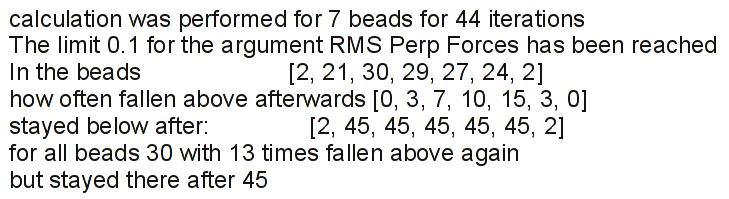
\includegraphics[scale=0.7]{Pictures/findlimitaofoutputethanoxid}

\caption{\textbf{Example output of tool find\_limit\_path (chapter \ref{sub:Findlimitaof.py}).
As one can see from the output the last iteration is indeed not the
best: the line stayed below, means that for all further iterations
the limit was never overstepped again. As it gave an argument larger
than the last iteration, this means that the last iteration had a
value over the searched one. The outermost beads are the not moving
ones, thus they are fortunately below the value from beginning. The
tool starts comparing only in the second iteration, as some values
have a zero as start in the first one, therefore the 2 may indicate
that its really the second or already the first iteration in which
the limit was met. In Iteration 30 all beads have RMS perpendicular
forces below the threshold, thus this is a much better result path
than the one of the last iteration.} \label{fig:Example-findlimitaof}}

\end{figure}

\begin{itemize}
\item On default all informations of interest are stored in the path.pickle
files. For each iteration there is one called string.debug?.path.pickle.
So the interesting one in our example is string.debug30.path.pickle.
First there is a chance to get the path in xyz-format, for direct
inspection. This can be done by the tool path2xyz (chapter \ref{sub:Path2xyz.py}).


\textit{paratools path2xyz string.debug30.path.pickle -b }

The outcome can be redirected to a file and visualized with jmol for
example (figure \ref{fig:Path-30}).

\item To extract now the transition state approximations on this path, the
tool ts\_and\_mods (chapter \ref{sub:Tsestandmods.py}) comes in handy.
The following command extracts the highest bead approximation and
for two different path descriptions (part \ref{sec:Approximations-for-the})
the spline and cubic variant. The spine and cubic variant with given
distance by string should in general gives the best result. But in
many cases the highest bead is just sufficient.


\textit{paratools ts\_and\_mods.py string.debug30.path.pickle 1 4}

The result is also a xyz format output, which could be further used.
(If called with option --m, ts\_and\_mods will also produce some modevector
variants, the one called frompath is especially for the spline and
cubic case well suited).

\end{itemize}
%
\begin{figure}[H]
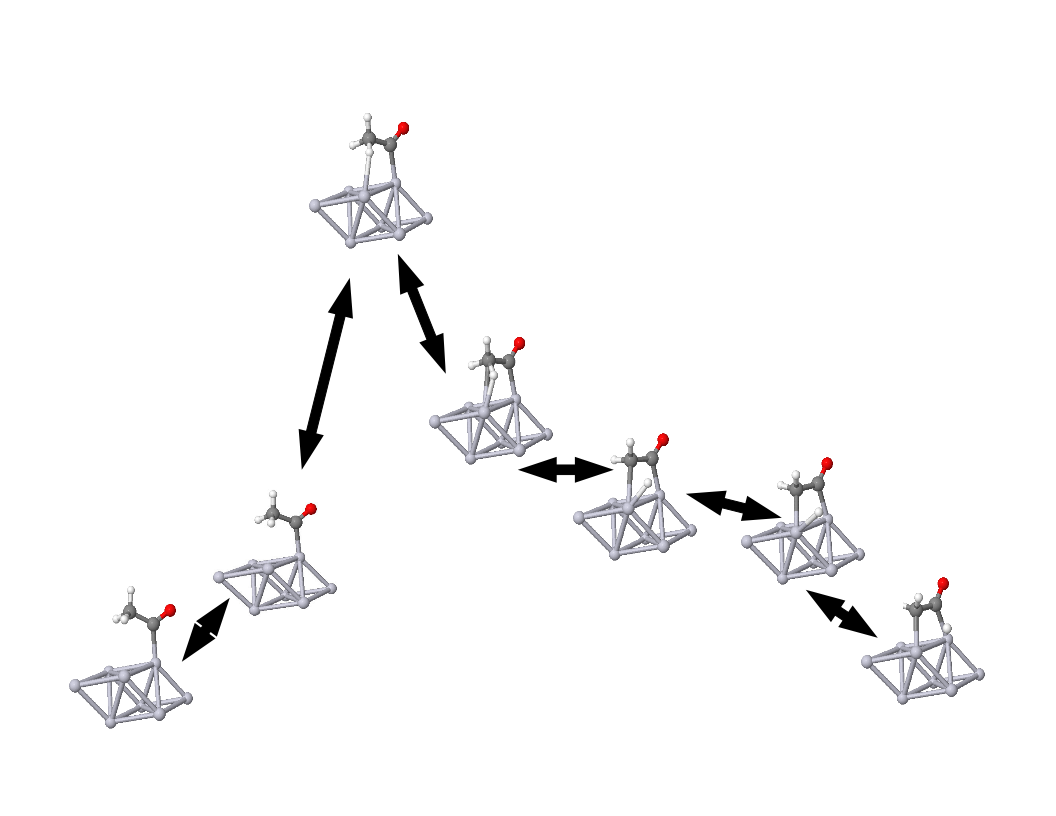
\includegraphics[scale=0.6]{Pictures/eo_30path}

\caption{\textbf{Path of the 30th iteration of the pathseracher. The geometries
in xyz format were extracted from the string.debug30.path.pickle file
with the tool path2xyz.}\label{fig:Path-30}}



\end{figure}


%
\begin{figure}[H]
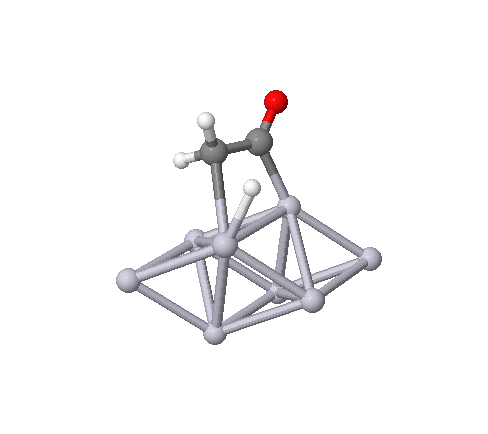
\includegraphics[scale=0.5]{Pictures/ethanoxidspacub}

\caption{\textbf{Transition state estimate. This one is produced with the variant
spine and cubic from the path of the 30th iteration of our minimal
energy path search with help of the tool ts\_and\_mods .}\label{fig:Transition-state-estimate.}}

\end{figure}


All this tools should now hopefully lead to a nice transition state
approximation, which will converge fast with any local transition
state searching tool. But there are a lot more tools and possibilities
of ParaTools. So let this chapter finish with just introducing two
more, which can be used also in the purpose of finding a transition
state, even if there had been no real turn for them in the recent
example.
\begin{itemize}
\item The toolbox has its own frequency calculation tool, which uses numerical
differences of the forces for approximating the needed hessian. The
description can be found in chapter \ref{sec:Parallel-Numerical-Frequency}.
Here it is also recommended to have a look at the parallel calculating
possibilities (part \ref{par:Parallel-Calculations}), as this tool
is highly parallelizable. Usage for the POSCAR.left of the example
above would be: 


\textit{paratools frequencies \nobreakdash-\nobreakdash-calculator
calc.py POSCAR.left}

Here the cell and fixed coordinates will be considered, too. This
is because they are stored in the POSCAR.

\item To watch the development of the path in special chosen internal coordinates
(independent of the coordinate system used for the path), there is
the tool path2plot (chapter \ref{sub:path2plot.py}). 


\textit{paratools path2plot --dp 2 8 7 10 --dis 2 5 string.debug0.path.pickle}

\textit{string.debug10.path.pickle string.debug20.path.pickle string.debug30.path.pickle}

The tool path2plot needs matplotlib to be installed. This might not
be available everywhere or the exact numbers are wanted. In this case
the tool path2tab can be used. It would give only the output for the
beads if not explicitly asked for an iterpolated path but in all other
things it should follow the same interface as path2plot.

\end{itemize}
%
\begin{figure}[H]
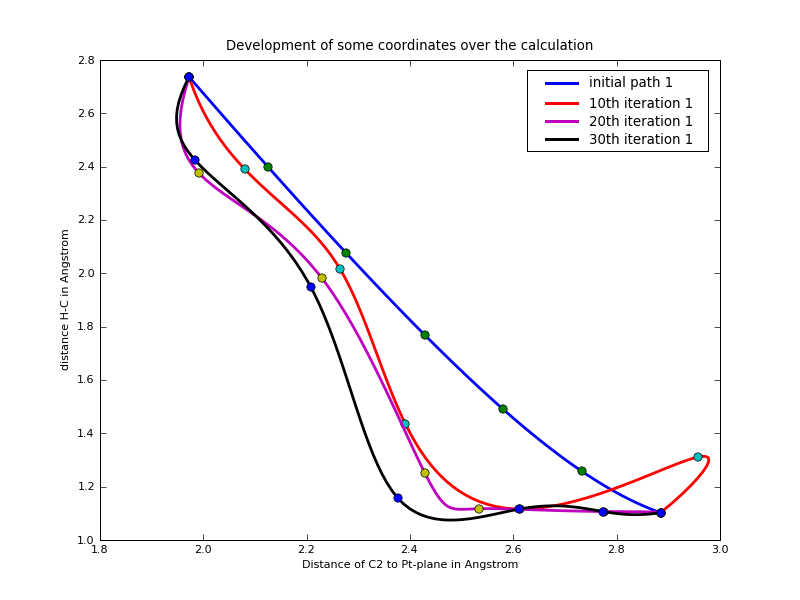
\includegraphics[scale=0.8]{Pictures/Ethanoxiddev_ito30}

\caption{\textbf{Development of internal coordinates. As a x-coordinate or
approximated {}``reaction'' coordinate there is the distance of
the second C atom to the Pt plane (the C which goes up), the y-coordinate
is the distance of the H atom to be dehydrated and the C atom bound
to. The tool shows the path and the beads as points on it. The picture
has been generated with the tool path2plot (see chapter \ref{sub:path2plot.py}).}
\label{fig:path2plot C-Ptpl H-C}}

\end{figure}


\pagebreak{}


\part{Different Functionalities of the Toolbox\label{par:Toolbox functions}}


\section{Some Functionalities of the Included ASE Toolbox}

The full functionalities of the ASE toolbox are described best by
their own manual. Here are only the parts, which are the most important
for \textcolor{black}{ParaTools:}


\subsection{The Atoms Object}

The atoms objects, as described in the ASE framework, are also used
to store molecules and atoms in ParaTools. Especially their interfaces
to the different quantum chemistry programs, called within ASE and
ParaTools as calculators, are important for ParaTools also. The atoms
contain all kind of data, like atom numbers, coordinates, forces,
energies, ...

The unit cell and the periodicity can also be found/set there.

Most of these data can be set or read in all the time. But of course
some kinds like atom numbers and atom symbols are connected and will
change also one another. 

The energies and forces are stored in the atoms object after one calculation
with any of the calculators. The coordinates are always updated after
they have been changed, by for example a minimization algorithm.

One way of defining atoms is:

\textit{co = Atoms('CO', positions={[}(0, 0, 0), (0, 0, 1.1)])}

But fortunately there is an even more simpler way: ASE can read in
several geometry formats and use them to generate atom objects by
extracting a lot of information from then. If not told otherwise it
will assume, that it had gotten a xyz-file. But if the name of the
geometry file includes {}``POSCAR'' or {}``CONTCAR'' it will try
to read them in as VASP format. In this case it assumes, that the
comment line in it will be filled with the atom numbers or a corresponding
POTCAR is at hand. One can also specify the format directly by specifying
it in the command. Thus the following two lines will both create an
atoms object from a POSCAR:

\textit{from ase import read}

\textit{min1 = read(\textquotedbl{}pos1\textquotedbl{}, format = 'vasp')}

\textit{min2 = read(\textquotedbl{}POSCAR2\textquotedbl{})}

Our own versions can also interpret gxfiles (needs gx in the name
or {}``format = 'gx''').

Most \textcolor{black}{ParaTools c}odes reading in geometries in one
way or another make use of this read function. Thus said codes can
be accessed with all formats valid for ASE.


\subsection{The Calculators\label{sub:The-calculators}}

One big advantage of having ASE in ParaTools is the amount of calculators,
which could be used. There exist wrapper around several important
quantum chemistry codes. So the geometry operations wanted can be
done with them. To learn more about the way the calculators have to
be used in ASE read the ASE manual. Here only the case of VASP will
be explained a bit further. ParaGauss (chapter \ref{sub:The-ParaGauss-Calculator})
and an extended VASP calculator (chapter \ref{sub:VASP-DFT-D-Calculators}),
as both are none of the standard calculators, will be explained more
in detail separately. The extended one adds also some DFT-D energies
to the VASP results. They cannot be found in the ASE documentations. 

\bigskip{}


In principle a calculator is also an attribute of an atoms object.
It is the wrapper around the quantum chemistry code and it could just
put in as:

\textit{calculator = Vasp( )}

\textit{min1.set\_calculator(calculator)}

This would be Vasp with the default values set by ASE. But there are
also some parameters which could be set or changed in addition. Thus
the calculator could also be initialized as shown in figure \ref{fig:Example-file-for-1}.

%
\begin{figure}[H]
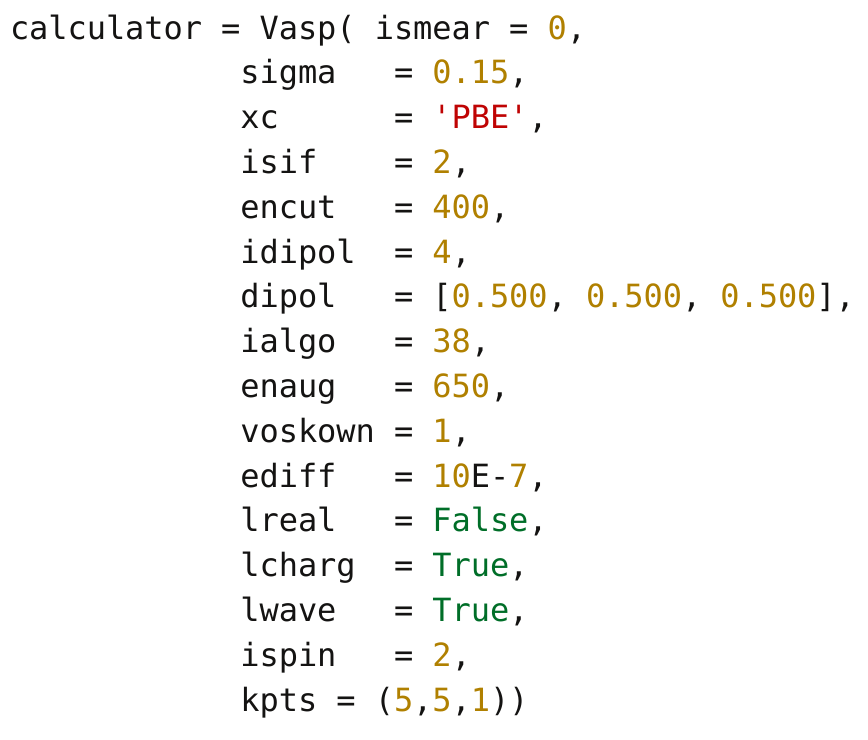
\includegraphics[scale=0.4]{Pictures/Calculator_new}

\caption{\textbf{Example file for containing a VASP calculator, most of the
variables which were special selected are common VASP variables. Note
the appearance of the kpts (k-points) which are normally specified
in a separate VASP input file. }\label{fig:Example-file-for-1}}

\end{figure}



\subsection{Geometry optimization}

Some rather useful features of ASE are the optimizers, for minimization
the forces on a geometry. There are several local optimizers and one
global one. The local optimizers are: BFGS, LBFGS, FIRE, MDMin, the
SciPy optimizers SciPyFminBFGS and SciPyFminCG and BFGSLineSearch.
The only global one right now is BasinHopping. The usage of them is
something like (with min1 an atoms object as above):

\textit{dyn1 = BFGS(min1)}

\textit{dyn1.run(fmax=0.01, steps=100)}

Which would start a minimization with BFGS method on the min1 geometry
till the forces are below 0.01 or 100 optimization steps is exceeded.
ParaTools provides also a wrapper to this methods in its central commaned
as {}``minimize''.


\section{Additional Calculators}


\subsection{The ParaGauss Calculator\label{sub:The-ParaGauss-Calculator}}

So far there exist only the possibility of using ParaGauss in the
ASE framework with help of the usual ParaGauss input file. But there
have to be made some adaptions to it, in order to run correctly:

The TASK is set to GeoOpt and the MAX\_GEO\_ITERATION (in the convergence
section) to zero: 

\textit{\&task}

\textit{task = \textquotedbl{}GeoOpt\textquotedbl{} }

\textit{... }

\textit{/task }

\textit{... }

\textit{\&convergence }

\textit{MAX\_GEO\_ITERATIONS = 0 }

\textit{...}

\textit{/convergence}

This is done to make ParaGauss calculate energies and forces and store
them in the gxfile. It will automatically force ParaGauss to take
the geometry from the ASE-generated gxfile and not from the input.
Thus the geometries specified in there need not be correct. MAX\_GEO\_ITERATIONS=0
on the other hand prevents the built-in optimizer of ParaGauss to
start and \textquotedbl{}consume\textquotedbl{} the energy/forces
in gxfile and overwrite it with updated geometry. There need not be
a gxfile at the beginning, the initial geometry will be provided by
ASE framework anyway. If there is a gxfile it must not be for a different
system (ASE will try to reuse the additional informations, as there
might be also the GxOptimizer working at the same time, which would
need them). 

If there is no need for the forces but only the total energy, there
is the chance to revert to energy calculations by specifying 

\textit{\&task }

\textit{task = \textquotedbl{}SinglePoint\textquotedbl{} }

\textit{read\_gx = true }

\textit{...}

\textit{/task}

Here ParaGauss has to be explicitly told to use gxfile for input geometry. 

There is no checking if the saved\_scfstate.dat is the right one,
so it has to be deleted before running on a different system.

The calculator is just invoked in ParaTools by the command.

\textit{calculator = ParaTools( )}

There are some parameters possible which might need to be reset:
\begin{itemize}
\item input: this is what ParaTools expect the input file of ParaGauss to
be named as. As default it is input.
\item cmdline: ParaGauss will be started by the command: 


\textit{cmdline input}

Therefore cmdline should contain the runpg version and the ParaGauss
executable. So for example:

\textit{cmdline = \textquotedbl{}runpg /users/alexei/exe/openmpi/mainscf\_V3.1.4b7-64\textquotedbl{}}

This expects runpg to be in a directory of path and to be use the
version V3.1.4b7 of ParaGauss used from the specified path. Cmdline
has also to be changed if parallel execution is wanted. 

\item silence: This flag indicates if ParaGauss's standard output is given
to standard output (False) or is stored in a separate file (True).
Be aware that the separate file will be overwritten if ParaGauss is
called several times in the same folder.
\item copy\_input: ParaGauss needs the input file and sometimes even some
other files in the subdirectory it will ultimately run. These subdirectory
might be different from the one in wich the calculator is created
and therefore the input file has been picked up. Furthermore several
instances of ParaGauss might be running in parallel, started from
the same calculator but with different input files (for example different
occupations set), which will somehow join their results lateron. Normally
ParaGauss would write the input file anew each time it starts a calculation
(copy\_input = {}``always''). Alternatively one can forbid him to
write input files (copy\_input = {}``never'') or allow only to write
them if they are not already there (copy\_input = {}``inexistent'').
Be aware that in the last case there can be a race condition if the
input is generated by another program while ParaGauss wrapper is running.
\item optimizer: Some ParaGauss single point calculations might want some
specifications of {}``optimizer.input'' like about the environment
ParaGauss should run in. As ParaGauss might be running in a different
subdirectory (as already mentioned) it might be convinient to ask
the Program to create this file also. If this is wanted ParaGauss
expects the optimizer parameter to specify the file, which should
be provided as optimizer input. The file itself needn't be called
optimizer.input but if it is not in the directory the ParaGauss wrapper
will be created in, the path to it has to be included also. Optimizer.input
will be created, if specified, in any case, thus independent of copy\_input
variable.
\end{itemize}

\subsection{VASP DFT-D Calculators\label{sub:VASP-DFT-D-Calculators}}

The calculator specified here is mainly an extension to the existing
Vasp calculator. It only adds to them empirical corrections to the
total energy for the noncovalent dispersion interactions. Thus all
the variables, which can be set in Vasp, can be set also here, compare
description for the ASE standard calculators in chapter \ref{sub:The-calculators}.
Thus the following example script is the minimal way of using it (as
it is a python example it needs to include the ase modules directly
by \textit{import ase}).

\textit{import ase}

\textit{system = ase.read('POSCAR.left') }

\textit{pbed = ase.calculators.Vasp\_d()}

\textit{system.set\_calculator(pbed) }

Additional the implementation provides the possibility to set an interaction
list, specifying for each atom to which interaction group it belongs.
As a default all atoms are in the same interaction group and interact
whith each other. The list can be specified directly. For the example
in figure \ref{fig:DFT+D}, it would look like:

\textit{system.interactionlist = {[}0, 0, 0, 0, 0, 0, 1, 1, 1, 1,
1, 1, 1, 1]}

%
\begin{figure}[H]
\textbf{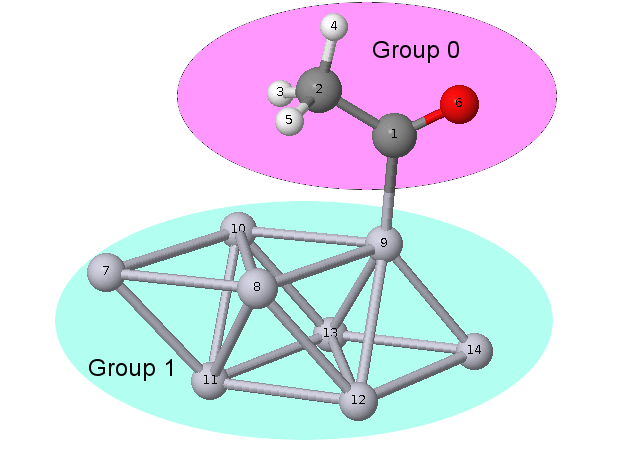
\includegraphics[scale=0.7]{Pictures/ethanox_numbered_2}}

\caption{\textbf{When applying the atoms can be assigned to different groups.
The interactions between the groups can then be defined separately.
In this example there are two groups, of which one refers to the surface,
while the other contains all the atoms o fthe adsorbate.}\label{fig:DFT+D} }

\end{figure}


There are specified two groups, the order of the atoms is given by
the numbers in the figure \ref{fig:DFT+D}. 

In this case only those interactions between atoms from different
groups will be considered. But if the interactions between the groups
should be specified other than in this default way, this can be done
by giving an additional interactionmatrix. This matrix tells if there
should be an interaction between two groups (by the number 1) or not
(by the number 0). Here the element in the n'th line and m'th column
specifies the interaction between the groups n and m. Of course the
interaction matrix should be symmetric.

Thus the default specification would be given by:

\textit{system.interactionmatrix = {[}{[}0,1], {[}1,0]]}

Another example would give also the interaction between adsorbate
atoms but not those of the surface:

\textit{system.interactionmatrix = {[}{[}1,1], {[}1,0]]}

To summarize things: to use the example system with adsorbate and
surface in different groups and not adding any surface-surface interactions,
one would have to write in the script:

\textit{import ase}

\textit{system = ase.read('POSCAR.left') }

\textit{pbed = ase.calculators.Vasp\_d()}

\textit{system.set\_calculator(pbed) }

\textit{system.interactionlist = {[}0, 0, 0, 0, 0, 0, 1, 1, 1, 1,
1, 1, 1, 1]}

\textit{system.interactionmatrix = {[}{[}1,1], {[}1,0]]}


\section{Different Kinds of Coordinate Systems\label{sub:coordinateSystems}}

%
\begin{figure}[H]
a)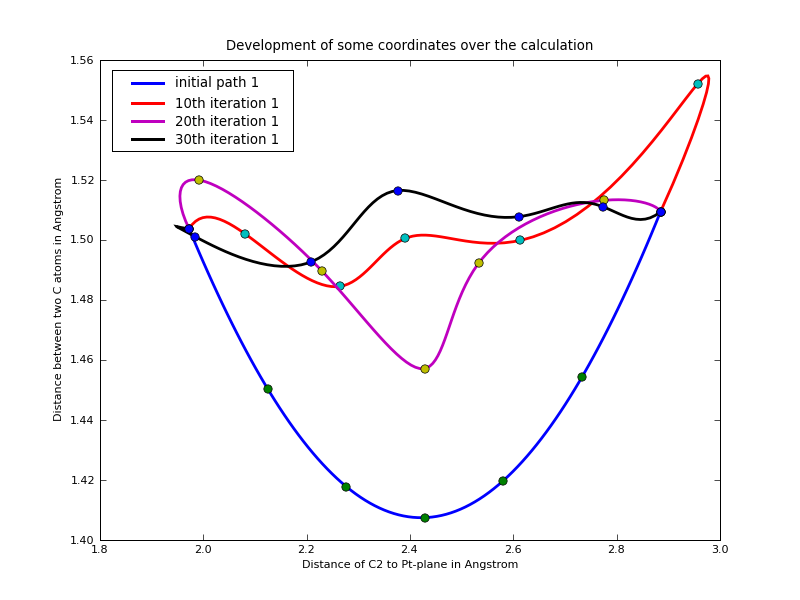
\includegraphics[scale=0.4]{Pictures/ethanoxiddevdsC}b)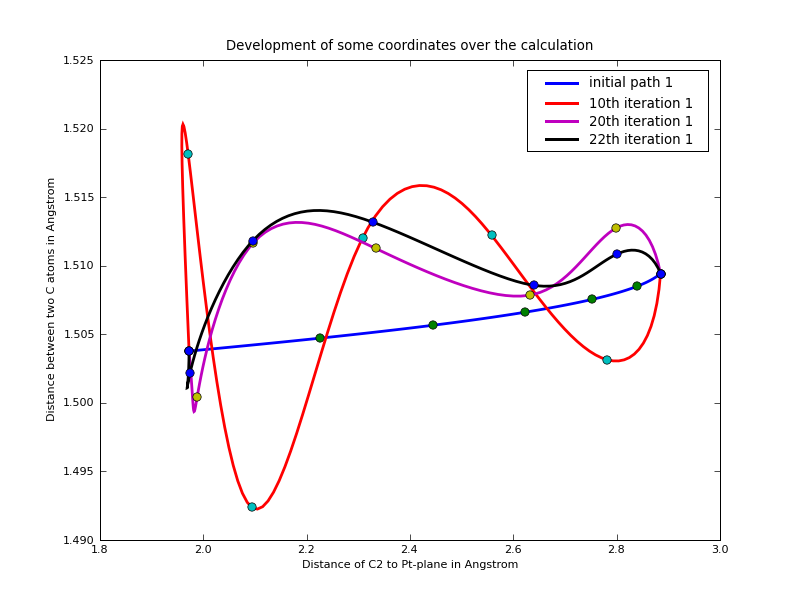
\includegraphics[scale=0.4]{Pictures/ethanoxiddevc2_mc}

\caption{\textbf{Some internal coordinates are not suppose to change too much
over time. Distance of the two C-atoms in the example of chapter \ref{sec:How-to-Find}.
a) Calculation of the C-atoms in Cartesian coordinates b) the distance
C-C is also a variable. Note the different scales of the pictures.
Here the linear interpolation of both seem not too fitting, but using
the right coordinate system may save time in faster calculations and
in some cases stop divergency. (Pictures were generated with tool
path2plot.py, chapter \ref{sub:path2plot.py} )\label{fig:Some-internal-coordinates}}}

\end{figure}


Several of the tools need coordinate systems. Generally ParaTools
should accept all kinds of coordinate systems but for the interactive
usage of the command paratools there are in general only three available:
Cartesians, internals and mixed ones, where mixed ones refer to a
system where parts are Cartesians and parts are internal. It really
depends, which is to be preferred for a given calculation. But in
some cases (see figure \ref{fig:Some-internal-coordinates}) using
other than Cartesian make the starting interpolation much smother,
giving better changes for a fast and correct convergence. The main
tools needing a special coordinate system are the pathsearching routines,
like neb or the different string methods (in \ref{sec:The-Path-Searching}),
the tool for just generating the path (see \ref{sub:Makepath.py})
or the Dimer and Lanczos methods for finding the transition state
( in \ref{sec:Dimer_Lanczos}).

The geometries will be always be provided by ASE readable geometry
files. They will contain Cartesian coordinates, from which the internal
and mixed coordinates can be created. But internal and mixed coordinates
need not be unique: this holds for dihedral angles and quaternions,
generated for global rotation by mixed coordinate systems (see \ref{sub:Mixed-Coordinates}
below) which have a $\pi$ periodicity. For interpolation between
two of thm there are therefore two different ways possible.


\subsection{Cartesian Coordinates}

Each atom has three coordinates, corresponding to a component in the
x, y and z-direction. In the ParaTools/ASE framework Cartesian coordinates
are in Angstrom. For ASE this is the only available coordinate system.
For the ParaTools routines they are the default. It is in some of
the routines possible to fix some of the coordinates, see details
in the tools. But as some of the geometry objects of ASE (like the
wrapper around VASPs POSCAR) might also contain some informations
about fixing of coordinates there is another way of getting this information.
Here ParaTools would only use this information from the ASE geometry
object if it did not got a direct input (a mask most certainly) for
it.


\subsection{Internal Coordinates\label{sub:Internal-Coordinates/zmatrix}}

The coordinates are described as distances, angles and dihedral angles
to other atoms. Of course this way the first atoms will not get as
many values as the others, as there are not enough other atoms to
create all the coordinates. Thus for n atoms there will be 3n-6 coordinates
(1 for n=2). 

\bigskip{}


The connectivities of the atoms amongst each are described with a
zmatrix and thus are given by the user. A complete zmatrix may look
something like:

$ $

\textit{Ar }

\textit{Ar 1 var1 }

\textit{Ar 2 var2 1 var3 }

\textit{Ar 3 var4 2 var5 1 var6 }

$ $

It defines the connectivities between the atoms. The first element
in a line is the atom symbol. The numbers of the atoms are given by
their line number, starting with 1. A line may be already finished
after the atom symbol. If not up to three variables follow, which
connect it to the atoms already defined. 

Thus a full line holds the informations: number of atom 1 (the new
defined one, through the line number), symbol for atom 1, number of
atom 2, name of variable for distance, number of atom 3, name of variable
for angle, number of atom 4 and name of variable for dihedral angle.
For the variables all the atom numbers specified before are used,
thus distance is between atom 1 and atom 2. 

The variable names in the zmatrix have in real only one purpose: they
show if some variables should be set to the same values. This they
can see by these variables have the same variable name. Be aware that
ParaTools does not try to find out if it makes sense to have the same
variables reused, at it will neither test if they belong to the same
categorie (distances, angles, etc.) or if they start with a similar
value. It is also possible to have a value of a variable (most certainly
an angle or dihedral angle) set to the negative of another variable.
In this case the second one should have the same variable name precceeded
by a minus symbol. The following example shows this: here all distances
are the same, while the two angles are the same absolute value but
with opposite signs:

$ $

\textit{Ar }

\textit{Ar 1 d1 }

\textit{Ar 2 d1 1 a1 }

\textit{Ar 3 d1 2 -a1 1 da1 }

$ $

The Zmatrix is given to the program normally, if not stated otherwise,
with the parameter\textit{ \nobreakdash-\nobreakdash-}zmat <name
of zmatrix file>. If several geometries are needed the zmatrix is
supposed to be valid for all of them. If it is possible to fix some
coordinates (like in pathsearcher or dimer method) the coordinates
are used from the zmatrix for it. They will appear always in the order
of the atoms. Be aware that three atoms have less coordinates than
the others.


\subsection{Mixed Coordinates\label{sub:Mixed-Coordinates}}

It is not needed to construct a zmatrix for all atoms if some internal
coordinates are wanted. The mixed coordinates allow to separate the
atoms in several groups, respectively several internal groups and
one Cartesian one. That there is only one Cartesian block at the end
is only a limitation of the ParaTools wrapper. Here each of the internal
coordinates block will also need some additional coordinates for a
complete description (remember that they specify for n atoms only
3n-6 coordinates, while Cartesians would 3n). They are about the orientation
of all the atoms in space, which is not given by the zmatrix. When
there are only internal coordinates they are not needed, but if there
is more than one block of atoms the positioning of each of these blocks
in the space becomes important as it defines how the atoms of different
blocks are connected. There are three variables for translation and
three for rotation (normally there would be only two rotation variables
for a block with 2 atoms, but in order to have the code as simplified
as possible there will be used also three of them for a two atom system.
The rotation of the object is described with quaternions. The additional
parameters have to be considered if some of the coordinates should
be fixed. After the internal variables of an internal coordinate block
the global orientation ones follow directly in the order translation
and then rotation variables.

ParaTools expect the order of the zmatrices and the atoms in the geometry
file to be connected with each other. If the first zmatrix defines
the coordinates for 4 atoms it will expect the first 4 atoms of the
geometry file to be the ones for the first internal coordinate block.
The global orientation variables of the atom group will position it
in the space exactly at the same position/orientation than was in
the geometry file. If after the atoms have been distributed on the
zmatrix-files there will be still some of them left, they will be
forwarded to the mixed coordinate system as Cartesians. As Cartesian
coordinates are already about global positions in the space, here
no additional objects for connecting them to the rest is needed. The
variables of this system will then be all the internal with their
global positioning variables and rest Cartesian coordinates together.

There is no possibility of getting a mask from the atoms object for
mixed coordinates, even not for the ones left in Cartesian.


\section{The Path Searching Methods\label{sec:The-Path-Searching}}


\subsection{Main Tool for Path Searching Calculations}

The tool pathsearcher is the general interface to the string and NEB
methods. It can be accessed via the paratools command, either with
directly selecting the method (like NEB, string, searchingstring)
or by the general command path-searcher. Then one can specify the
method in the parameter settings as method.

Usage:

\textit{paratools path-searcher \nobreakdash-\nobreakdash-calculator
<calculator filename> GEOM1 GEOM2}

For either string or NEB methods one needs to specify at least two
geometries and the calculator. 

\textit{paratools searchingstring \nobreakdash-\nobreakdash-calculator
<calculator filename> GEOM1 GEOM2}


\subsubsection{Geometry\label{sub:Geometry_path}}

There are three different kinds of coordinate systems valid in ParaTools,
they are described in more detail in chapter \ref{sub:coordinateSystems}. 

The geometries should be provided as files. Valid file formats are
all those, that can be interpreted by ASE. This includes xyz-, POSCAR-,
and gx-files. File format is in part determined from the file name
or extension, e.g. POSCAR and gx-files by the presence of \textquotedbl{}POSCAR\textquotedbl{}
or \textquotedbl{}gx\textquotedbl{} substrings. See \ref{sub:Geometry-Parameter}
for more details.

\bigskip{}


A method of getting an internal (or mixed coordinate system) is by
giving the geometries in Cartesian (or as ase-files) and specifying
only the zmatrix or zmatrices once. Each of them will then be set
by writing\textit{ \nobreakdash-\nobreakdash-zmatrix <zmatrix file}>.
It will then be read in from there and used to generate zmatrix or
mixed coordinate object. The function can recognize by its own, that
there are fewer variables than needed and fill up with Cartesian ones. 

\bigskip{}


A zmatrix may look something like:

$ $

\textit{C}

\textit{H 1 var1 }

\textit{H 1 var2 2 var3 }

\textit{H 1 var4 2 var5 3 var6 }

\textit{H 1 var7 2 var8 4 var9}

$ $

The chapter \ref{sub:coordinateSystems} gives some more information
on coordinates and zmatrices. It is also possible to have several
coordinates set to the same value by reusing the variable name.


\subsubsection{Geometry Parameter\label{sub:Geometry-Parameter}}

Some special parameter handle the interpreting of the geometries.
They can be set exactly the same way as the other parameters. The
calculator is also formally one of them, as it decides what energy
and forces belong to a given program. Others might be required by
periodic programs.
\begin{itemize}
\item cell:	the cell in which the molecule is situated, needed for example
by Vasp
\item pbc:	which cell directions have periodic boundary conditions
\item format: ParaTools (throught ASE) know several formats for geometry
files. If some of them a provided it tries to identify them. But this
is done only by the name of the geometry. If it for example is POSCAR.1
it will recognise the POSCAR in it and interprete it as Vasp POSCAR
file; if it finds gx in the name it expects gxfile and so on. If it
does not find anything in the name it still process the files, expecting
xyz files. However if one wants to choose its name free from any limits
of ASE interpreting one can provide the format directly here and be
fine with any names (expect if they start with --). The format {}``xyz''
would enforce for example also POSCAR.1 to be read as xyz-file, {}``vasp''
will accept everything as POSCAR and {}``gx'' will expect a gxfile.
Check the ASE manual for a complete list of available formats and
their names.
\item mask: which of the given geometry variables are supposed to be changed
(True) and which should stay fix during the calculation (False). It
should be a string containing for each of the internal variables the
given value. As the default all variables are optimized (this is indicated
by mask = None). Will be explained more in detail in \ref{sub:Fixed-Coordinates}
\item calculator:	the quantum chemistry program to use, like Vasp or ParaGauss;
Only indirect in the command line usable, as here it should name a
separate calculator file, in which the calculator is set, it will
be explained in \ref{sub:Calculator}
\item zmatrix: Uses the n first not already used atoms for generating the
internal coordinates for n atoms as specified in the zmatrix. More
details in \ref{sub:Geometry_path} , \ref{sub:Internal-Coordinates/zmatrix}
and \ref{sub:Mixed-Coordinates}. 
\end{itemize}
For some of this set of parameter there is a second way of obtaining
a new value for them: The ASE atoms objects may contain more information
than only the chemical symbols and the geometries of the wanted object.
For example in POSCARs there are additional information about the
cell (pbc would be also set automatically to true in all directions)
which ASE could understand. This information can also be accessed
by ParaTools. If they are available, they are only used, if these
variables still contain the default parameters after setting all other
parameters. Additionally ASE can access some constraints, which may
be taken from a POSCAR or can be set directly. Some of them can be
also used to generate a mask. This is only done if Cartesian coordinates
are used. 


\subsubsection{Calculator\label{sub:Calculator}}

The calculator can be given in ASE format. It can be set in the paramfile
or in an own file (for example calc-file) via.

\textit{\nobreakdash-\nobreakdash-calculator <calculator file>}

Additionally one can use some of the default specified calculators
by for example: 

\textit{\nobreakdash-\nobreakdash-calculator default\_vasp}

The calculators can be set up the same way as described in chapter
\ref{sub:The-calculators}. There is no need to connect the calculator
with anything. But therefore it is absolutely needed, that the name
of the calculator is calculator, even if in general cases, as in chapter
\ref{sub:The-calculators}, where it is used directly it could have
been given any valid unused name.


\subsubsection{Fixed Coordinates\label{sub:Fixed-Coordinates}}

There is the possibility to fix variables with the mask option. Here
one has to say explicitly which coordinates should be fixed. This
is done by giving a list, containing an entry for every variable.
The entry would be {}``False'' for a fixed variable or {}``True''
otherwise.

As a default no coordinates are fixed. 

But despite the chance of giving them directly there is also another
option in case of Cartesian coordinates: there may be already some
information in the atoms object, which stores the geometry information
of the minima. It could be set there directly, but it is more common
to expect it to comes from the input file. In POSCARs for example
one may use {}``selective dynamics'', which fixes some of the coordinates.
These informations can be interpreted from ASE as constraints, which
then can be used from ParaTools to fix some coordinates. For general
usage with the constraints (via python code): ParaTools can interpret
the {}``FixScaled'' and the {}``FixAtoms'' constraints of ASE.
ParaTools only fixes coordinates this way if they are the only mask
available and if only Cartesian coordinates are used.


\subsubsection{Parameter Defining Pathsearcher Behavior}

There are some other parameters specified, which decide on how the
program will run. There is a list of default parameters, which also
includes some parameters for the geometries (see subsection \ref{sub:Geometry-Parameter}).
These defaults can be accessed by:

\textit{paratools path-searcher \nobreakdash-\nobreakdash-defaults}

They can be changed in two different ways:
\begin{itemize}
\item By including in the parameters of the calculation the following:


\textit{\nobreakdash-\nobreakdash-paramfile <filename>}

All the variables could be set in the file filename. 

\item Or by giving them directly as options to the paratools call:


\textit{\nobreakdash-\nobreakdash-<parameter to change> <new value>}

So for example:

\textit{\nobreakdash-\nobreakdash-ftol 0.01}

This does not work for all variables but most of them can be also
provided thus.

\end{itemize}
If the same variable is set in both the paramfile and directly, the
directly set value is taken.

An example: 

\textit{\nobreakdash-\nobreakdash-name NewName} 

would set the name to NewName in the parameters.

\bigskip{}


There exists: (Parameter: short description directly)
\begin{itemize}
\item method:	 what calculation is really wanted, like NEB, string, growingstring
or searchingstring, only needed if the path-searcher is started, \textit{paratools
string} and so on will set it on their own.
\item opt\_type:	what kind of optimizer is used for changing the geometries
of the path, as default the new multiopt is used for the string methods,
while for NEB it is reset to ase\_lbgfs
\item pmax:	maximal number of CPUs per bead
\item pmin:	minimal number of CPUs per bead
\item cpu\_architecture:	 describes the computer architecture, which should
be used; normally contains the number of processors the calculation
should run as a python string (so for example \textit{cpu\_architecture
= {[}8]} for 8 processors)
\item name:	the name of the calculation, appears as basis of the names for
all the output; needn't be set: as a default it takes the method as
name
\item beads\_count: 	how many beads (with the two minima) should be used;
growingstring and searchingstring start with less, for them it is
the maximum number of beads. The two beads representing the minima
(which are not optimized) are also calculated here, thus \textit{beads\_count
= 4 }means two beads will be optimized.
\item ftol: 	the force convergence criteria, calculation stops if RMS(force)
< ftol 
\item xtol: 	the step convergence criteria, only used if force has at least
ftol {*} 10 
\item etol: 	energy convergence criteria, not really used 
\item maxit: 	if the convergence criteria are still not met after maxit
(maximum iteration) iterations, the calculation is stopped anyhow
\item maxstep: 	 the maximum step a bead can take during optimization
\item spring: 	the spring constant, only needed for NEB
\item output\_path: 	place where most of the output is stored. The working
directory is not filled up too much, as all output goes there. Default
is subdirectory {}``\textit{workplace}''
\item output\_geo\_format: ASE format, in which the output-geometries of
the last iteration are written; it is xyz as default, but can be changed
for example to gx or vasp (POSCAR)
\item output\_level:	the amount of output is decided here, for more information
see list below
\end{itemize}
Pmax, pmin and cpu\_architecture should be adapted to each other.

The following parameters can only be specified in the parameter file.
But they are not much used anyhow.
\begin{itemize}
\item placement:	executable function for placing processes on beads, only
used for advanced calculations
\item pre\_calc\_function:	function for precalculations, for calculator
Gaussian etc.
\end{itemize}
\bigskip{}


The output\_level has the following valid values:
\begin{itemize}
\item 0: minimal output; not recommended; provides only logfile, geometries
of the beads for the last iteration (named BEAD?) and the output needed
for the calculation to run.
\item 1: reduced output; additional to output of 0 there are the ResultDict.pickle
(usable for rerunning or extending the calculation without having
to repeat the quantum chemical calculations) and a path.pickle of
the last path; the path.pickle may be used as input for some other
tools, it stores the \textquotedbl{}whole\textquotedbl{} path at it
is in a special format. 
\item 2: recommended output level (default): additional a path.pickle for
every path is created; these path.pickle files can be easily accessed
by several of paratools other tools and allow to quicker get informations
of the path they represent. If not only the last result of the calculation
is of interest but also the development these files make it much easier
to access all the data.
\item 3: some more output in every iteration, for debugging etc. 
\end{itemize}

\subsubsection{Reuse Results from Previous Calculations }

It is possible to store the results of the quantum chemical calculations
(which are the computational most expensive part of the calculation)
in a ResultDict.pickle file. It is done by default for an output level
with at least 1. If a calculation with the same system should be done,
or the calculation should be repeated, these results can be reused
(the QC- program mustn't be changed, as well as atoms used). To reuse
this results the parameters cache is used:

\textit{\nobreakdash-\nobreakdash-cache <filename>}

filename should be directed on the file (with location) where the
Results are stored, thus the old ResultDict.pickle file. 

ParaTools will then append the given ResultDict.pickle file instead
of creating a new one. It is also possible to give ParaTools a non-existing
ResultDict.pickle as input for \textit{cache}. This will then created
at the specified location with the given name instead of using the
default values here. If the \textit{cache} variable is not given but
ParaTools finds a ResultDict.pickle at the location where it wants
to create its storage it will delete this file first, expecting it
to be not valid.


\subsubsection{Initial Path\label{sub:Initial-Path}}

The minimal input required for generating an initial path are the
two minima, which should be anywhere there. Then the path-searcher
codes wil use as initial path an linear interpolation in all the variables
of the two minima. But this path may be totally off. First in calculations
with periodic boundary conditions one has to ensure that none of the
atoms is in different cells in the two geometries. But this may not
be sufficient. Linear interpolated atoms might show completly unchemical
behavior as tunneling through a surface instead of moving around its
edge. This might make it unusal hard or even impossible for the path-searcher
routines to converge towards the real path.

In this cases there is the chance of giving some additional geometries,
which should be on a better initial path. 

In internal coordinates there might apppear another problem: Not all
internal variables are uniquely defined by the Cartesian geometries.
Dihedral angles and the quaterions describing the global rotation
for parts of a mixed system have a $\pi$ periodicity. The path-searcher
will take as a default the shortest possible path in them. But if
the longer one (with the norm of dihdral angles larger than $\pi$
between the minima) are wanted there is need for giving some more
informations on the inital path. Note that the reduction on angles
smaller than $\pi$ is only done between succeeding geometries, thus
the comlete path may go over bigger angles. This reduction is only
done at the beginning before the first path is generated. During the
optimization the affected angles may of course grow over $\pi$. But
it is not very likely that the system will converge to the path rotating
the other direction than has been chosen as inital path. 

\bigskip{}


There are different ways of setting an initial path. One of the additional
files generated with output level 3 is a state\_vector, which can
be given directly as input for\textit{ \nobreakdash-\nobreakdash-init\_path
state\_vec.} This would than in the next calculation let it start
with the path described by this. Such an state vector may be also
generated by hand. It is a file containing for all the points on the
path (might be different bead number than in the wanted calculation)
the values for all internal coordinates.

If such a state\_vec is not available one can also provide the initial
path by giving the additional geometries directly in the same format
as the two minima. In this case the call of the method would be something
like:

\textit{paratools path-searcher \nobreakdash-\nobreakdash-paramfile
<filename> minima1 bead2 bead3 bead4 minima2}

or for a minimal example:

\textit{paratools searchingstring \nobreakdash-\nobreakdash-calculator
calc.py POSCAR? POSCAR??}

The number of initial points and beads need not be the same.


\subsubsection{Examples}

A minimal one would be:

\textit{paratools searchingstring \nobreakdash-\nobreakdash-calculator
default\_lj left.xyz right.xyz}

A more advanced one:

\textit{paratools path-searcher --method string \nobreakdash-\nobreakdash-paramfile
params.py \nobreakdash-\nobreakdash-ftol 0.07 \nobreakdash-\nobreakdash-name
Hydration POSCAR? POSCAR??}

Here one needs several POSCARs for the initial path. A parameter file
(called params.py) should hold some parameters, so especially the
calculator. But whatever is inside, ftol is anyway 0.07.


\subsection{The Direct Call of NEB/String with Interactively Command}

The commands 

\textit{paratools neb ...}

\textit{paratools searchingstring ...}

and so on are just shortcuts for 

\textit{paratools pathsearcher \nobreakdash-\nobreakdash-method
neb ...}

and

\textit{paratools pathsearcher \nobreakdash-\nobreakdash-method
searchingstring ...}

Therefore pathsearcher is the general name for all these tools in
this manual.


\subsection{Interpreting the Output of a Path Searching Calculation\label{sub:Interpreting-the-Output}}

The output consists of several files, which will be explained in the
current chapter. The standart output is more or less debug informations,
the only interesting part of it is, if it anouces at the end {}``Optimization
converged'' or {}``Optimisation STOPPED (maximum iterations)\textquotedbl{}.
The output for string, growingstring , searchingstring and even neb
is in principle the same. Note only that the names of the files normally
resemble the name of the calculation, thus {}``string'' for a string
calculation and {}``growingstring'' for a growingstring calculation.
The differences are mainly a varying bead number for growingstring
and searchingstring against a fixed one for string and neb. In the
following the output will be explained for a string calculation (with
Vasp were informations about the calculator are needed). 


\subsubsection{The Logfile}

\noindent The main information can be found in the .log file, in the
example named string.log. It summaries the information of the string
in the i'th iteration. One of these iteration can be found between
the \nobreakdash-\nobreakdash-\nobreakdash-\nobreakdash-\nobreakdash-\nobreakdash-\nobreakdash-
and ====== separators. For each iteration there are several sections.
The first section therein contains informations about the whole string,
summarized or averaged over all the beads:

\noindent \textit{VALUES FOR WHOLE STRING}

\noindent \textit{Total Energy : -548.2954 }

\noindent \textit{RMS Forces (perp|para) : 1.9747 | 1.2268 }

\noindent \textit{Step Size (RMS|MAX) : 0.0000 | 0.0000 }

\noindent \textit{Cumulative steps (max bead) : 0.0000 }

\noindent \textit{Cumulative steps (ts estim) : 0.0000 }

\noindent \textit{Bead Sep ratio (Pythagorean) : | 1.0018 }

The total Energy is the sum of the energies of all beads, RMS Forces
is the RMS over the forces of the moving beads. The Step size is calculated
from the step of all beads as well. 

\bigskip{}


The second section contains the values for the single Beads:

The Bead Energies here are the values for the related bead, note that
the 4'th bead gives in this example the highest value. (compare also
figure \ref{fig:Energy-from-the})

%
\begin{figure}[H]
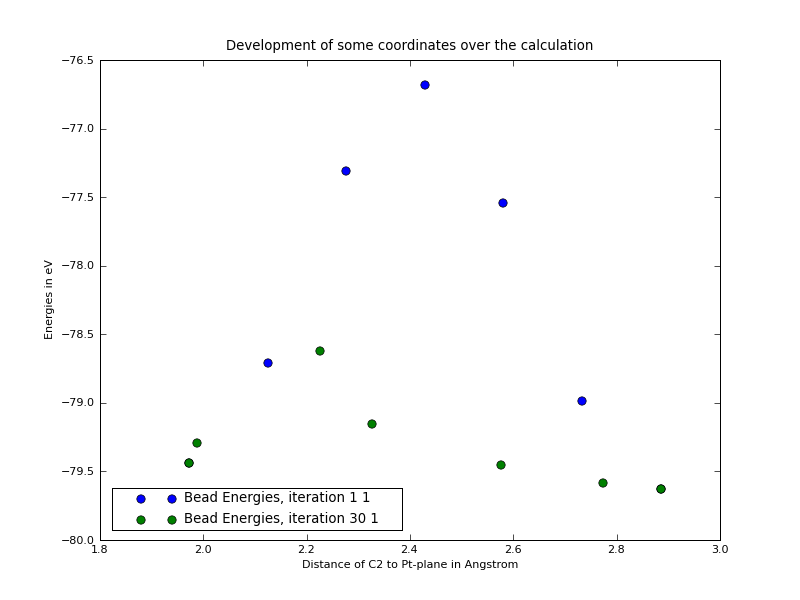
\includegraphics[scale=0.8]{Pictures/EthanoxidEnergy}

\caption{\textbf{Energy from the logfile for the example from chapter \ref{sec:How-to-Find}.
The plot was done with help of the tool path2plot.py (chapter \ref{sub:path2plot.py}).
The relaxation of the Energy from the first to the 30th iteration
is shown. Here it is only possible to display the energies on the
beads, as there is in general no path over the energies obtained.\label{fig:Energy-from-the}}}

\end{figure}


The RMS Perp Forces are perpendicular to the path, the RMS Para Forces
are parallel to the path. The first ones should vanish at convergence.
Thus a reduction in said forces indicates that the string methods
is working fine. The Step Size in the first iteration is of course
everywhere zero, it should vanish also towards the end. The Bead Angles
are calculated between the different beads. When starting with a linear
interpolation they are always 180, but later on they change a lot.
If they become too small, there may be a problem with 'kinks' in the
path. The Raw State Vector gives the value for all variable Coordinates
changing during the calculation. It uses here its 'internal coordinates',
which can be Z-Matrix coordinates, flattended Cartesian coordinates
or mixed coordinates. Be aware that it only gives values for Variables,
so if in the complete description of the system some variables are
fixed they do not appear here. 

\textit{VALUES FOR SINGLE BEADS }

\textit{Bead Energies : -79.6284 | -78.9829 | -77.5451 | -76.6803
| -77.3100 | -78.7066 | -79.4421 }

\textit{RMS Perp Forces : 7.970e-03 | 1.505e+00 | 2.271e+00 | 2.444e+00
| 2.138e+00 | 1.236e+00 | 1.283e-02 }

\textit{Para Forces : -1.243e-02 | -1.533e+00 | -1.761e+00 | -1.628e-01
| 1.573e+00 | 1.608e+00 | -2.962e-03 }

\textit{MAX Forces : 1.786e-02 | 3.546e+00 | 5.095e+00 | 5.454e+00
| 4.125e+00 | 2.745e+00 | 3.183e-02 }

\textit{RMS Step Size : 0.000e+00 | 0.000e+00 | 0.000e+00 | 0.000e+00
| 0.000e+00 | 0.000e+00 | 0.000e+00 }

\textit{Bead Angles : | 180 | 180 | 180 | 180 | 180 | }

\textit{Bead Separations (Pythagorean) : | 7.960e-01 | 7.975e-01 |
7.970e-01 | 7.960e-01 | 7.970e-01 | 7.975e-01 }

\textit{Bead Path Position : 0.000e+00 | 1.665e-01 | 3.333e-01 | 5.000e-01
| 6.665e-01 | 8.332e-01 | 1.000e+00 }

\textit{Raw State Vector : }

\textit{Coordinate 1 : 4.4599 | 4.3823 | 4.3046 | 4.2269 | 4.1493
| 4.0716 | 3.9939 }

\textit{Coordinate 2 : 2.4377 | 2.3359 | 2.2341 | 2.1322 | 2.0305
| 1.9287 | 1.8268}

\textit{...}

\bigskip{}


The third section holds general information of the calculation:

\textit{GENERAL STATS }

\textit{Callbacks : 1 }

\textit{Number of respaces : 0}

\textit{Beads Count : 7 }

\textit{Total Length (Pythag|Spline) : 4.7810 4.7810 }

\textit{State Summary (total) : 7.2466 }

\textit{State Summary (beads) : 7.4697 | 7.3882 | 7.3105 | 7.2368
| 7.1674 | 7.1022 | 7.0413 }

\textit{Barriers (Fwd|Rev) : 2.9481 | 2.7617 }

Here one finds how often there has been an iteration accepted (Callbacks)
and how many beads there are (currently). It will also tell how often
since start the beads have been respaced. The rest are some less important
informations about the bead, which were put apart from the first sections.


\subsubsection{Files after finished calculation\label{sub:Files-after-finished}}

After the string calculation has finished it generates some files
about the last path, considering it somehow as its result (at least
for output level > 0). These files can be both understood by humans,
but also read in again by some tool. As in this context they are mostly
containing only numbers the name of the file should say everything
about the contenst already. There is {}``internal\_coordinates'',
containing the last bead coordinates. Here the same coordinates, which
are shown in {}``Raw State Vector'' of the logfile are given (in
Angstroms or radients). Another one, {}``abscissa'', contains their
positions on the path for path parameterizing, thus the first value
should there always be 0 and the last one 1. As the beads needn't
be equal spaced in the path varialbe, not even (completely) for a
plain spline interpolation this information might be valuable for
further observations of the path. As these values do not exist for
neb calculations where the spacing is done by the spring forces, a
neb calculation will not create this file. The file {}``energies''
contains as it says the energies of the beads (in eV) and {}``forces''
the corresponding first derivatives (in eV/Angstrom) to Cartesian
coordinates.

The Cartesian coordinates of the beads are used to generate xyz-files,
which could be easily read in by jmol or other visualization tools.
They are named bead<i> for the i'th bead. If wanted they could contain
also the information in one of the other geometry formats ASE could
understand. This can be archived by accordingly setting the parameter
{}``output\_geo\_format'' to the ASE shrotcut for the wanted format. 

The ts\_estimate<i> files contain the geometry of approximated transition
states. As ParaTools expects that the search with the string methods
was done as a step for getting the transition state. The approximation
used here is the {}``spline and cubic'' method, compare chapter
\ref{sub:Available-Methods-TS}. Only if it fails the highest bead
method is used. The output is the same as for the bead<i>. The internal
coordinates (as in logfile given) are printed to the corresponding
ts\_internals<i>.


\subsubsection{The Path.pickle File}

The string.path.pickle file contains all informations of the last
path in an ParaTools readable format (not human readable through).
Thus it can not be used directly, but the toolbox provides a lot of
other nice tools, which uses this as an input. So for example the
other transition state estimate methods can be extracted from it.
The tools should accept also other formats of the input, like the
files in \ref{sub:Files-after-finished}, but then in general more
than one file is needed and it has to make clear to the method which
file is which. The path.pickle file is an elegant way to move the
information in a simple form. On the other hand path.pickle files
are more sensible. They are not longer readable any more if the format
changes or the python code changes its pickling methods too much.
Thus they are more something for the direct following observations,
not for long time savings of the results.


\subsubsection{Other Output }

If the output\_level is raised, more output appear: for output\_level
= 2 each path iteration generates a path.pickle file. They are situated
in the working directory and are called string.debug<i>.path.pickle.
If after the finished calculation the development of it should be
observed or of a crashed calculation a path should be recreated they
are quite useful. For output\_level = 3 there will be the state\_vec
files for each iteration (as mentioned in the initial path chapter
\ref{sub:Initial-Path}). There will be also some CoS.log's (for each
iteration) which contains the path in an ASE readable format. For
this level there will also appear some archive in the logfile.


\section{Local transition state searcher: the Dimer/Lanczos method\textcolor{red}{\label{sec:Dimer_Lanczos}}}

These methods belong to the class of eigenmode following methods.
To be a bit more exact, first they try to determine the eigenvector
corresponding to the lowest eigenmode of the Hessian matrix, than
they perform a step uphill this direction and downhill in all others.
They update their idea of the eigenvector after each step on the energy
surface. The steps on the energy surfaces are normally called translation
steps, while for dimer the update steps are normally called rotation
steps. In the following we will use these notations also for the Lanczos
method, even when here the term {}``rotation'' is not really fitting.
The difference between Dimer and Lanczos is merely the way how this
eigenvector is calculated. In all other respects they are the same,
using the same interface. Except when differences are explicitely
mentioned as in \ref{sub:Differences-between-Dimer/Lanczos} the explanations
are holding for both methods, even when they are only mentioning Dimer.


\subsection{The required input for a Dimer/Lanczos method}

A minimal usage would look something like:

\textit{paratools dimer --calculator <calculator file> <geometry file>
<start mode vector file>}

Other than the reaction path search there is only one input geometry
\textit{<geometry file>} required. The file and all geometry relevant
parameters to interprete it are interpreted exactly the same way as
it described for the pathsearcher routine in \ref{sub:Geometry_path},
\ref{sub:Geometry-Parameter} and \ref{sub:Fixed-Coordinates}, with
the only limitation that for dimer we have only one of those files.
Also the calculator, which defines the quantum chemical program to
use is interpreted over the same interface as for the path searcher
routines in \ref{sub:Calculator}.

But additionally a direction is needed as \textit{<start mode vector
file>} (some kind of mode vector). This direction is the start value
for the eigenvector search. Here one should note that the methods
are not supposed to calculate all eigenvalues for the Hessian matrix.
Thus they have no possibility to check if the eigenvector they have
found really belongs to the minimal eigenvalue or is a higher one.
Therefore one should avoid giving them a start mode vector which points
in a eigenvector direction, which is not the smallest one. The mode
itself is given as a file, containing a value for either every internal
geometry variable (also Cartesians are interpreted as internal geometry
if they are the only specified system, but do not forget that fixed
coordinates are not appearing here) or a Cartesian block of $N_{\textrm{Atoms}}\times3$,
which then has to contain a value for all Atoms (also if all their
coordinates are fixed).


\subsection{Differences between Dimer/Lanczos method\label{sub:Differences-between-Dimer/Lanczos}}

Both methods are about finding a special mode, the one belonging to
the smallest eigenvalue of the approximated Hessian. For this the
dimer method sets up two images around its current geometry (one at
+ mode\_vector {*} dimer\_distance and the other at - mode\_vector
{*} dimer\_distance) then it rotates them around their midpoint till
the convergence criteria are met (Implemention details prefer to use
one such image and the midpoint, only approximating the second image).
The Lanczos method is a direct method for eigenvalue determining.
Here the quantum chemical calculations are done to build up a basis
in a subspace. In this subspace eigenvalues and eigenvectors of the
reduced Hessian are calculated. If the smallest one of them has a
direction which (up to a convergence criteria) is also an eigenvector
in the complete space it is supposed to be the mode vector.

Both methods use a start vector for their iterations and both will
converge rather fast if the start vector is very near the wanted result.
Especially with the more rouher convergence criteria they should perform
very similar. However if a very exact result is needed Lanczos usually
outperforms Dimer. Lanczos needs at least the number of degrees of
freedom, as in this case the subspace would collapse to the complete
space. Thus if it is not converged after this amount of times, this
should be a problem of rounding errors and the not ideal quantum chemical
calculations, as it is supposed that the Hessian is exactly represented
by differences in the gradients regarding the midpoint. If more than
the number of degrees of freedom are used the Lanczos method might
get severe problems generating a new basis vector (which should be
orthogonal to all the others) and thus might crash.


\subsection{The parameters of the Dimer/Lanczos method\label{sub:parameter_Dimer}}

Like for the pathsearcher routine there are two different ways of
setting variables, directly in the command line or specified in ap
parameterfile, which is then given as:

\textit{--paramfile <name of paramfile>}

In this file the parameters are given as <name> = <value>, where strings
(consisting of letters have to given with {}``''). Thus in such
a file one could find the line:

\textit{trajectory = {}``every''}

All the parameter to set can be seen with

\textit{paratools dimer --defaults}

However there are some more parameters to stear the dimer method with.
They are about implementation details and thus normally not required
to be changed. If they should be accessed anyway one can set as first
parameter of the dimer method \textit{--accept\_all}. This will remove
the restriction on only known parameters for dimer. Be aware that
this way there will be no checking of any of the parameter really
exists. The dimer method accepts any parameter and just ignores everything
it does not understand.

Parameter which are explicitely free for adaption are:
\begin{itemize}
\item max\_translation: Maximal number of translation steps (be aware that
before each translation there will be the rotation step, thus this
is not the number of gradient calculations.
\item max\_rotations: How many rotation steps for each translation step
are allowed. Be aware that for the Lanczos method it only makes sense
to have here at maximum the number of degrees of freedom of the system,
as here a subspace of that order is build. If more are used (during
run time) the system might crash.
\item max\_gradients: Another way of setting a limit to the general steps
of the system. The gradient calls of rotation and translation step
are called and sumed up and used as abortion criteria. Be aware that
said criteria is checked in the translation steps only, thus it is
possible to have up to max\_gradients + max\_rotations steps before
the system terminates.
\item trans\_converged: The criteria for translation step and thus for the
complete algorithm. The absolute maximum of the gradients is tested. 
\item phi\_tol: Convergence criteria for the rotation step. It is tested
as an angle in radiens: for Dimer the angle the system would rotate
in the next step (or an early approximation); for Lanczos the angle
between current and last mode approximation or the angle between mode
vector and its approximated gradient (means mode vector is eigenvector)
can stop {}``rotation''
\item max\_step: Maximal step length for the translation step.
\item trajectory: While the calculation proceeds the geometry and the modevector
will be changed continuously. This parameter is now about how much
of this can be found lateron in the subfolder the calculation runs
in. All geometry files given for the trajectory are in xyz-format,
the modes contain a matrix of floats. All the files are human readable.
There are different leves given as a string:

\begin{itemize}
\item newest: only the actual geometry and the actual mode\_vector are given
in the files actual\_geometry and actual\_mode. This is also the default.
\item empty: No geometry or modes will be stored.
\item every: for each iteration n the geometry and the mode are stored to
geo<n> and mode<n>
\item one\_file: the actual geometry is given as for newest. Additionally
all the geometries and modes are stored in two big files, all\_geos
and all\_modes. All\_geos just contains the geometries one after another
as this way some programs can read it in as a path; the modes in all\_modes
are separated by a line {}``Mode of iteration <n> {}``
\end{itemize}
\end{itemize}
It is strongly recommended to set at least the max\_translation or
the max\_gradients as the default is very near running forever.


\subsection{Interpreting the output of a Dimer/Lanczos method}

There is only few output of the dimer method. The parameter trajectory,
explained in \ref{sub:parameter_Dimer} is already responsible on
how many files will be created. All the other output goes to the standard
output. Here one gets a per (translation) step information and a result
information, after the method has finished. The start of such output
might be something like this:

\textit{Intermediate steps for translation and rotation informations }

\textit{Values are in eV, Angstrom, degrees or combinations of them }

\textit{Trans. Infos: Energy ABS. Force Max. Force Step: Perp\textbackslash{}Para
Angle to mode }

\textit{Rot. Infos: Conv. Steps. curvature Angle to last }

\textit{Step 0 with sum of Grad. calcs. 5 }

\textit{Trans. Infos: -5353.12736 8.63831 5.67751 0.10000 0.09052
\textbackslash{} 0.04251 64.84407 }

\textit{Rot. Infos: True 1 -51.91102 59.85055 }

\textit{Step 1 with sum of Grad. calcs. 10 }

\textit{Trans. Infos: -5399.74253 6.90785 4.04526 0.10000 0.09389
\textbackslash{} 0.03443 69.86065 }

\textit{Rot. Infos: True 1 -86.99553 17.38904 }

\textit{Step 2 with sum of Grad. calcs. 15 }

\textit{Trans. Infos: -5401.94974 5.48020 3.55572 0.10000 0.09962
\textbackslash{} -0.00871 85.00543 }

\textit{Rot. Infos: True 1 -62.44341 10.41689 }

\textit{Step 3 with sum of Grad. calcs. 20 }

\textit{Trans. Infos: -5381.29876 5.43350 3.82003 0.10000 0.09993
\textbackslash{} -0.00379 87.83059 }

\textit{Rot. Infos: True 1 -38.45217 10.78196 }

\textit{Step 4 with sum of Grad. calcs. 24 }

\textit{Trans. Infos: -5405.85113 2.63210 1.52607 0.10000 0.09967
\textbackslash{} 0.00813 85.33809 }

\textit{Rot. Infos: True 0 -33.00477 0.00000 }

\textit{Step 5 with sum of Grad. calcs. 29 }

\textit{Trans. Infos: -5426.61526 4.22819 2.80965 0.09195 0.09165
\textbackslash{} 0.00750 85.32368 }

\textit{Rot. Infos: True 1 -36.71423 8.33504 }

The first four lines are there for explaining the step information.
The step information consists of three lines, which are repeatet for
each step. The first saying {}``Step 4 with sum of Grad. calcs. 24''
gives the current translation step number and the sum of all gradient
calculations done till this step. The other two lines starting with
{}``Trans. Infos:'' and {}``Rot. Infos:'' belong to the corresponding
lines in the start input. They give the informations named there.
Thus about the translation we have the informations: 

\textit{Trans. Infos: Energy ABS. Force Max. Force Step: Perp\textbackslash{}Para
Angle to mode }

\textit{Trans. Infos: -5353.12736 8.63831 5.67751 0.10000 0.09052
\textbackslash{} 0.04251 64.84407 }

\textit{Trans. Infos: -5399.74253 6.90785 4.04526 0.10000 0.09389
\textbackslash{} 0.03443 69.86065 }

\textit{Trans. Infos: -5401.94974 5.48020 3.55572 0.10000 0.09962
\textbackslash{} -0.00871 85.00543 }

\textit{Trans. Infos: -5381.29876 5.43350 3.82003 0.10000 0.09993
\textbackslash{} -0.00379 87.83059 }

\textit{Trans. Infos: -5405.85113 2.63210 1.52607 0.10000 0.09967
\textbackslash{} 0.00813 85.33809 }

\textit{Trans. Infos: -5426.61526 4.22819 2.80965 0.09195 0.09165
\textbackslash{} 0.00750 85.32368 }

\textit{Trans. Infos: -5412.94735 3.23080 2.30023 0.10000 0.09982
\textbackslash{} 0.00598 86.57346}

Thus the first entry in the lines is the energy of the current image,
the second the absolute Force followed by the maximum (absolute) force.
The length of the step is followed by the length of the step compontents
perpendicular and parallel to the current mode vector. Angle to mode
describes the angle between step and mode vector. The max force compontent
is used for determining convergence, it should be vanish by a successful
calculation at the end. The different step components and the angle
to the modevector allow to see which part of the step belongs to the
minimization and which to the steps in direction of curvature. The
same can be done for the rotation informations:

\textit{Rot. Infos: Conv. Steps. curvature Angle to last }

\textit{Rot. Infos: True 1 -51.91102 59.85055 }

\textit{Rot. Infos: True 1 -86.99553 17.38904 }

\textit{Rot. Infos: True 1 -62.44341 10.41689 }

\textit{Rot. Infos: True 1 -38.45217 10.78196 }

\textit{Rot. Infos: True 0 -33.00477 0.00000 }

\textit{Rot. Infos: True 1 -36.71423 8.33504 }

\textit{Rot. Infos: True 0 -30.41641 0.00000 }

\textit{Rot. Infos: True 1 -31.35842 5.92447} 

First it is told if the rotation is converged, followed by the number
of steps used for it. The curvature of the eigenmode should become
negative soon and stay thus. Be aware that the method does a step
against the mode direction if the curvature is positive (in this case
the corresponding Trans. Infos should show only a parallel step).
This should help by leading the system faster away from a minimum.
The angle is to the mode vector of the last iteration.

\bigskip{}


After the calculation has terminated, the first line will tell if
it has converged or not. Then follows a section:

Results as given back from dimer routine

This section gives all informations which the dimer method has stored
(many only about the last iteration). As it is not yet clear if the
dimer output will be sufficient in the future, this section might
help to recover additionally needed informations. 

The real Result is given in the section {}``Results DIMER calculation'':

\textit{Results DIMER calculation: }

\textit{Dimer converged: True }

\textit{Forces left (RMS): 0.000182624417635 }

\textit{Number of gradient calculations: 539 }

\textit{Mode at last iteration: }

\textit{{[} -5.76549663e-02 -1.41683844e-04 -7.38774329e-01 -3.48719225e-02
-1.36373646e-05 1.64732136e-01 3.39781235e-01 1.26865209e-04 6.45620463e-02
-2.19727913e-01 -3.40441112e-04 5.04614323e-01]}

\textit{Final geometry: }

\textit{4}

\textit{\smallskip{}
}

\textit{C 0.086343848074545 -0.000236223361009 -0.023510946078905 }

\textit{O 1.254608644091847 -0.000218171587174 0.001129852669768 }

\textit{H -0.522219646394556 -0.000226903373099 -1.608140932787113 }

\textit{H -0.965375148654632 -0.000249550524969 -0.362765373052858}

This section starts again with the information if the calculation
has finished. Especially if this is not the case the gradients left
on the last image might be of interest. It tells how many gradient
calculation has been done during the complete run. Additionally it
gives the last mode and of course the last geometry. This in a xyz
style independant of the internal coordinates used.


\section{Additional Tools for the Path Searching (on Output Files)}

The following tools are designed for interpretation of a finished
path searching with one of the path\_searcher routines. They are working
on some output of it. Many of them make use of the the path.pickle
files. Some of them accept also a replacement input but this is much
more complicated as they work with several files. 


\subsection{Seeing Error of Approximation to Real Transition States}

The tool pp2ts-err tells how far is a given transition state-estimate
from the true transition state, if the later is known. This tool is
mainly good for debugging. 

Usage: 

\textit{paratools pp2ts-err {[}options] file.pickle {[}ts-actual.xyz] }

Options:
\begin{itemize}
\item -t: find TS approximation from path
\item -g: gnuplot output 
\item -m: display modes 
\end{itemize}

\subsection{Transition State Estimates on Path\label{sub:Tsestandmods.py}}

%
\begin{figure}[H]
a)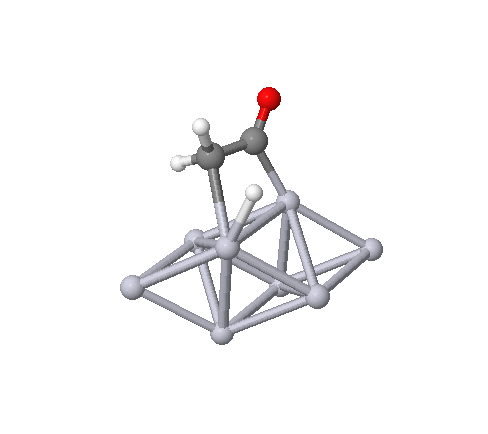
\includegraphics[scale=0.5]{Pictures/ethanoxidhighest}b)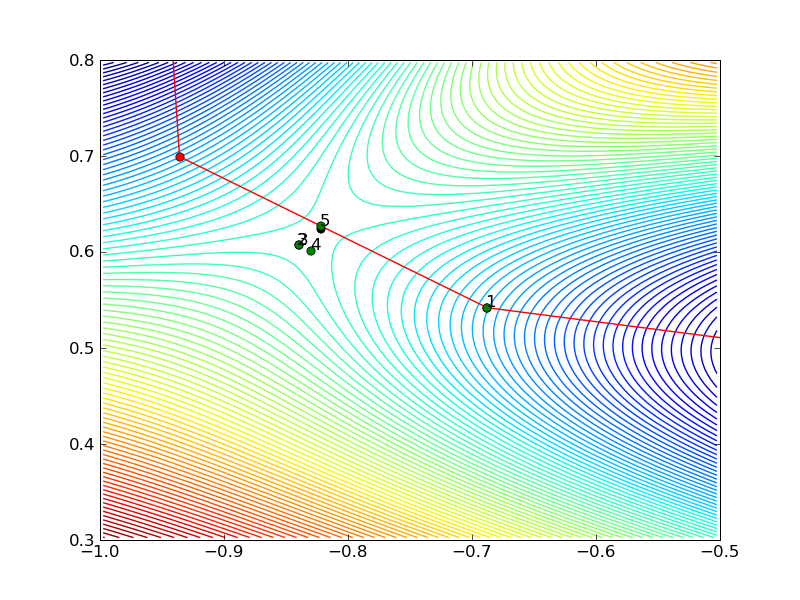
\includegraphics[scale=0.4]{Pictures/smallest15}

\caption{\textbf{Sometimes the highest bead is not enough as transition state
estimate. a) highest bead approximation for our system from chapter
\ref{sec:How-to-Find}. b) different transition state approximations
from a path (red) on a Mueller-Brown surface. The transition states
are numbered, but not in the order of their estimate number. It is
easy to see, that there are some differences, and that the highest
bead (number 1) is in this case not the best. The tool Tsestandmods.py
can generate all the transition states in an easy way and allows also
to compare the forces left on the structures. \label{fig:Sometimes-the-highest}}}



\end{figure}


The tool ts-and-mods takes a path.pickle file and estimates the transition
states from it. It can be also used with different input, like the
user readable files created from path\_searcher after convergence.
Gives back the transition states (and the modevectors) for different
transition state estimates. First argument is the path.pickle or geometry
file to read in (or \textit{\nobreakdash-\nobreakdash-help} to get
a help text). Compare figure \ref{fig:Sometimes-the-highest}. The
usage is something like:

\textit{paratools ts-and-mods file.path.pickle }

One can choose which transition state estimates are to be generated
by giving the numbers related to the wanted ones (default is all of
them).


\subsubsection{Different input way}

In the usage without path.pickle the the path.pickle file is exchanged
by a file containing the geoemtries in internal coordinates for all
beads (like the internal\_coordinates file of path\_searcher). But
in oder to be able to work it needs not only the geometries but also
some more informations:

One has to add in the parameters \textit{\nobreakdash-\nobreakdash-s
<symbolfile> <energyfile> <forcefile>}. These are the files which
are needed at least to create the input.\textit{ <symbolfile>} should
contain all the atom symbols (of one image), separated by whitespace;\textit{
<energyfile>} and \textit{<forcefile>} the energies and forces on
all bead positions (this should be just the same format than the one
given in the files for energies and forces for the last iteration
of the path\_searcher.

Additionally one make want to give the abscissa of the beads in a
file. This is done by \textit{\nobreakdash-\nobreakdash-a <abscissafile>.}
A NEB calculation would not use abscissas at all and thus not create
this file but the string calculations will provide it for the last
path. 

The geoemtries of the internal\_coordinates are internal ones. The
tool might therefore need to know how to interprete them. As default
it supposes them to be Cartesian ones. But if the calculation has
been done in internal coordinates or with a mask, they have additionally
be given here. For internal or mixed coordinates just provide the
zmatrices as done for the main calculation as \textit{\nobreakdash-\nobreakdash-zmat
<zmatrix file>. }The mask should be also available in a separate file
and here a complete image of the system before the mask was used is
needed, so a geometry file without masked set (but only for one geometry).
These informations can be provided by \textit{\nobreakdash-\nobreakdash-mask
<mask file>} \textit{<geometry for unmasked system>}.


\subsubsection{The Different Transition State Estimates}

\begin{tabular}{|c|c|}
\hline 
number & TS-estimate\tabularnewline
\hline
\hline 
1 & highest\tabularnewline
\hline 
2 & Spline\tabularnewline
\hline 
3 & Spline and average\tabularnewline
\hline 
4 & Spline and cubic\tabularnewline
\hline 
6 & Bell method\tabularnewline
\hline
\end{tabular}

$ $

All the different transition states and the procedures behind can
be found in detail in \ref{sec:Approximations-for-the}. In short
it may be noted that the Spline and cubic is supposed to be the best
one; it is also used as output for the transition state estimates
for the path\_searcher in its last iteration. But often it is just
enough to take the highest bead.


\subsubsection{Other Arguments}

Other possible arguments:
\begin{itemize}
\item \nobreakdash-\nobreakdash-p : print the resulting transition state
estimates (is also the default if no other argument is set)
\item \nobreakdash-\nobreakdash-m : print also available mode vector estimates
(can also be given by any combination of p and m) 
\item \nobreakdash-\nobreakdash-f {[}<filename>]: calculates the forces
on each transition state estimate and gives also their projection
on the mode vectors (the calculator, which is used, is stored in the
path.pickle already). By default the \nobreakdash-\nobreakdash-p
option is set false. The following argument can be the name of a file
to write the forces and energies to, which may be reused for later
calculations. The file's name should not be a number or start with
\nobreakdash-\nobreakdash- . The file need not be there, then all
the output goes to standard output.
\item \nobreakdash-\nobreakdash-ff {[}<filename>]: like f but the output
of the comparison is printed to an external file energyandforce.dat.
\item \nobreakdash-\nobreakdash-r <stored forces file>: the next argument
has to be the name of a file to read the forces from. It is only useful
together with the \nobreakdash-\nobreakdash-f option. If it is set,
the program will look in the forces file, if there is already a calculation
for the current approximation (note that it will not check for any
other correspondence) and then use it instead doing a new calculation.
Missing forces will be calculated as before. The file should be look
like energyandforce.dat generated with the \nobreakdash-\nobreakdash-ff
option.
\item \nobreakdash-\nobreakdash-c {[}<logfile> <number of iteration>]:
for comparing the strings with the previous ones. This option is mainly
for debugging. The path, which is build by the transition estimation
tool may differ from the one used for minimization. This difference
should be very small compared to convergence arguments. This tool
gives as output relevant data from the approximated string(s). The
\nobreakdash-\nobreakdash-p option is set to false by default. If
the next argument is a file name (for a logfile) the program searches
in it for data to compare the results with. In this case it needs
also as an additional argument a number, saying which iteration to
take from. 
\end{itemize}
Except for the \nobreakdash-\nobreakdash-ff option all output goes
by default to the standard output.


\subsection{Showing Abitrary Internal Coordinates Along a Path\label{sub:path2plot.py}}

The tools path2plot and path2tab are the main routines of a whole
bunch of tools extracting informations from a path.pickle file and
make them understandable to the users. Both tools can handle also
the other input format but then are not that effective. They will
give some preselected internal coordinates or energy/gradient informations
and can also add some from a logfile. Path2plot will show a picture
of them (compare figure \ref{fig:path2plot}), path2tab will give
the data as a table to the standard output. Path2plot will need matplotlib
installed, which path2tab does not. As input there has to be some
path.pickle file(s) and at least two internal coordinates. Usage of
it:

\textit{paratools path2plot --dis 1 2 string.path.pickle --dis 1 3 }

\textit{paratools path2tab --dis 1 2 string.path.pickle --dis 1 3 }

%
\begin{figure}[H]
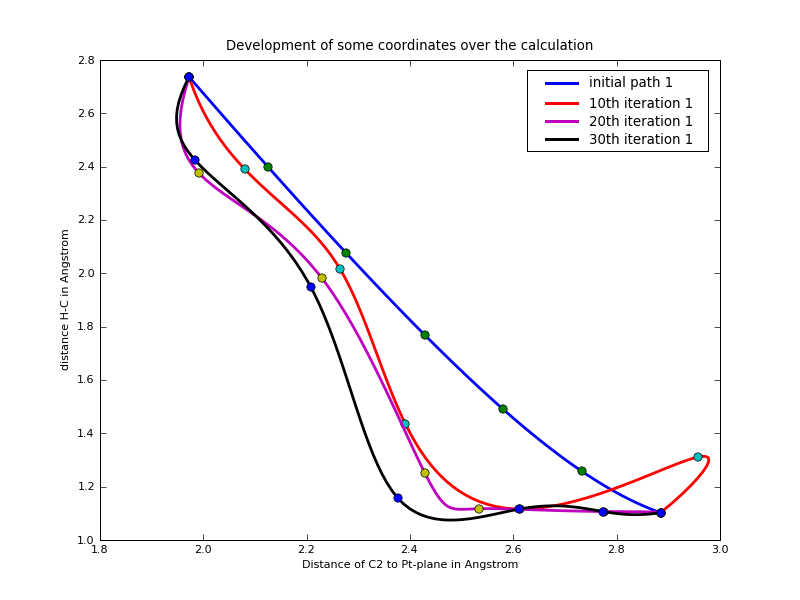
\includegraphics[scale=0.8]{Pictures/Ethanoxiddev_ito30}

\caption{\textbf{Path2plot is designed to show selected internal coordinates
(or variables from the .log file) in a graphical way. It allows to
see how the path in the given variables looks like. Watch out for
too steep drops, loops and such kinds to find out how good your given
path is. The picture here shows two internal coordinates from the
example given in chapter \ref{sec:How-to-Find} for three iterations.
The number 1 after the name of them is there if several values, like
several angles are looked at the same time.\label{fig:path2plot}}}

\end{figure}


First the shared part of the interface is described, followed by the
individual parts. The similar tools are described aditionally.


\subsubsection{Shared interface path2plot/path2tab}

There are two different ways of putting the main input into the routine:
the path.picke file contains all the informations required but as
in tool ts-and-mods in \ref{sub:Tsestandmods.py} it is also possible
to give it in internal geometry files. They can be of the kind the
path\_searcher creates as internal\_geometries. Then it is required
to provide the symbols in a separate symbolfile, in which they are
separated by whitespace. This file is given once as \textit{\nobreakdash-\nobreakdash-symbols
<symbolfile> }and will be used for all geometryfiles provided. If
the coordinates used in the calculation weren't raw Cartesians ones
it is also needed to tell the routine how they should be interpreted.
This can also be done once for all the geometry files. Zmatrix coordinates
are introduced in the same way as in the path\_searcher routine as
\textit{\nobreakdash-\nobreakdash-zmat <zmatrixfile>, }where\textit{
<zmatrixfile>} is the file with the connections and parameter definition,
which should be available from the current calculation. If a mask
has been used it has to be given also in a separate file, followed
by a geometry file containing the internal coordinates of all (also
the masked) coordinates. This geometry file should contain the geometries
of a single image and all but the masked values might be Nonesense
(0.0 for example). They are provided as \textit{\nobreakdash-\nobreakdash-mask
<maskfile> <geometry file>} to the tool. If availabe also abscissa
files should be provided. They are necessary to generate the same
path that was used in string calculations, while NEB does not know
anything about them. They needn't be given but here it is either none
or one for all, which means there should be exactly as many files
as for the internal geometries, where the n'th abscissa file will
belong to the n'th geometry file. They are provided as \textit{\nobreakdash-\nobreakdash-abscissa
<abscissafile>}.\bigskip{}


As variables of interest there are first of all the internal coordinates:
An internal coordinate is selected by settings \textit{\nobreakdash-\nobreakdash-<kind>
<n1> <n2>} ... where the ni's are the atom numbers (starting with
1) which should be used for getting the internal coordinate. How many
ni's are required is dependent on the kind of coordinate chosen. It
is also possible to abbreviate the kind by a number, also given in
the table below. 

These are the possibilities:

$ $

\begin{tabular}{|c|c|c|c|}
\hline 
internal coordinate & kind & number of Atoms needed & kind (number)\tabularnewline
\hline
\hline 
distance & dis & 2 & 2\tabularnewline
\hline 
angle & ang & 3 & 3\tabularnewline
\hline 
angle not connected & ang4 & 4 & 4\tabularnewline
\hline 
dihedral angle & dih & 4 & 5\tabularnewline
\hline 
distance to plane & dp & 4 & 6\tabularnewline
\hline
\end{tabular}

$ $

In the distance to plane the atoms defining the plane must not be
on a line.

Another possibility of selectable variables concern energies and gradients.
The results for the beads are given in the path.pickle file and are
extracted from there, if needed at another position they will be approximate
by a spine through the values for the beads. These coordinates are
only availabe for inputs of path.pickle files as reading in extra
files for energies and forces only to give the values back nearly
unchanged does not make much sense. For the energies all that can
be done is given them back, while of the gradients some different
values can be extracted. The names for the options are the following:
\begin{itemize}
\item \nobreakdash-\nobreakdash-energy or \nobreakdash-\nobreakdash-en
will process the energies
\item \nobreakdash-\nobreakdash-gradients or \nobreakdash-\nobreakdash-gr
will give the absolute value of the gradients
\item \nobreakdash-\nobreakdash-grmax will give the maximal value of the
gradients in internal coordinates
\item \nobreakdash-\nobreakdash-grpara gives the length of the gradient
component parallel to the path
\item \nobreakdash-\nobreakdash-grperp gives the length of the gradient
component perpendicular to the path
\item \nobreakdash-\nobreakdash-grangle gives the angle in degree between
the gradients and the path vector 
\end{itemize}
\bigskip{}


There are other options which may be set:
\begin{itemize}
\item \nobreakdash-\nobreakdash-diff : of the next two internal coordinates
the difference will be taken, instead of the values of each of them
\item \nobreakdash-\nobreakdash-expand <cellfile> <expandfile> : there
will be considered also some atoms, which are located in another cell.
The way they are generated is described below separately.
\item \nobreakdash-\nobreakdash-log <filename> <string> <num> : reads
in filename which should be the main output file of a string or NEB
calculation (the .log file) and takes string line of the num'th iteration
as some extra bead data. The needed x-values for this plot are the
same x-values as from the beads of the last path.pickle file given
before this option
\item \nobreakdash-\nobreakdash-lognf <filename> : new log as before,
but reuses the string and num argument from the last one. Only the
logfile is changed to filename.
\item \nobreakdash-\nobreakdash-lognn <num> : new log plot as above, but
takes another iteration than the last one.
\end{itemize}
\bigskip{}


The expand option needs some further explanation: To use it there
is need of two additional informations for the system: 
\begin{itemize}
\item The cell should be known. Thus for each of the three vectors of the
cell, the x, y and z-component should be given, in order to know how
much to shift in which direction. These informations are stored in
the cellfile. It has to be a file and should contain the unit cell
in the following format:


\textit{v11 v21 v31}

\textit{v12 v22 v32}

\textit{v13 v23 v33 }

The format is the same as used for unit cells all over ParaTools and
ASE.

\item Then the atoms which should be shifted have to be given: thus four
additional information per shifted atom have to be provided. They
are stored in expandlist, where each atom has the following format:


\textit{n a1 a2 a3}

This means that for atom number n there should be a replicate, which
is shifted a1 {*} v1, a2 {*} v2 and a3 {*} v3 in the three cell directions.
The shifted atom will have the number N + sn, with N being the number
of atoms in the original description and sn being the number of the
line of the atom in expandlist. 

\end{itemize}
The new shifted atoms can being accessed the same way as the others
just by their number.


\subsubsection{Only for path2plot}

Path2plot takes the first internal coordinate given as x-Value and
plots all others against it as y-value. Energy and gradient and lines
from the logfile are always given after the internal coordinates.
It is needed to povide at least one internal coordinate for the x-Value.

The following options are only availabe for the tool path2plot. They
are mainly about how the figure should be plotted:
\begin{itemize}
\item \nobreakdash-\nobreakdash-name <string> : string will be the name
of the path-plot. If there are several files the names could be given
by repeatedly set \nobreakdash-\nobreakdash-name <string for i>.
But in this case the name of the i'th call of \nobreakdash-\nobreakdash-name
option always refers to the i'th file, no matter in when the option
is set.
\item \nobreakdash-\nobreakdash-title <string> : string will be the title
of the picture 
\item \nobreakdash-\nobreakdash-xlabel <string> : string will be the label
in x direction 
\item \nobreakdash-\nobreakdash-ylabel <string> : string will be the label
in y direction 
\item \nobreakdash-\nobreakdash-logscale <z> : for z = 1,2 or z = x,y:
sets scale of this direction to logarithmic
\end{itemize}

\subsubsection{Only for path2tab}

Here all the data, no matter how many are given as a table. Energies,
gradients and logfile lines are always given after the internal coordinates
as well. There is only one option left to explain: in general path2tab
would return the values for the beads of the path.pickle or geometry
files. But it is also possible to tell him by the option \textit{\nobreakdash-\nobreakdash-num
<number>} to interpolate a path and give the interpolated values for
\textit{<number>} equal spaced images on it.


\subsubsection{Path2xyz\label{sub:Path2xyz.py}}

The tool path2xyz takes a path.pickle file reads it in and gives a
string of jmol type xyz-files to the standard output. They are equally
spaced in the path coordinate.

As a default it will give as many pictures as there were beads in
the path.pickle file, but any other number N can be given instead.

Run:

\textit{paratools path2xyz string.path.pickle N}

or simply:

\textit{paratools path2xyz string.path.pickle}

One could also demand to give back the beads in this format. The beads
my differ from the equally in the path coordinate spaced points, thus
this is different to running it without option. This could be done
by:

\textit{paratools path2xyz string.path.pickle -b }


\subsubsection{Xyz2tabint}

This program reads xyz files and gives as output the value of specific
coordinates of interest (they should be somewhat internal ones). A
list of all the coordinates of interest have to be provided. The parameter
accepted are:

\nobreakdash-\nobreakdash-ii <filename>: filename should contain
a list of specific coordinates of interest. Each coordinate should
have its own line.

\nobreakdash-\nobreakdash-id <num> <list> : direct input of the
list of specific coordinates, here num gives the number of coordinates
of interest in advance, then the list follows.

\nobreakdash-\nobreakdash-help : shows a help text.

\nobreakdash-\nobreakdash-degree : angles are given in degree, else
in radians

\nobreakdash-\nobreakdash-expand <cellfile> <expandlistfile>: if
another atom of a neighboring cell is wanted, this option helps to
work with a {}``shifted'' atom.

Usage:

\textit{paratools xyz2tabint --id 2 dis 1 2 dis 1 3 path.xyz}

\bigskip{}


The list of coordinates of interest should contain for each wanted
coordinate: first a number or abbreviation saying what kind of coordinate
is looked at. Then should follow the numbers of the atoms (in the
order of the xyz file) involved. 

The kind of coordinates can be extracted from the following table.

$ $

\begin{tabular}{|c|c|c|c|c|}
\hline 
kind & number & abbreviation & num atoms & specialty\tabularnewline
\hline
\hline 
distance & 2 & dis & 2 & distance a-b\tabularnewline
\hline 
angle & 3 & ang & 3 & angle a-b-c\tabularnewline
\hline 
 & 4 & ang4 & 4 & angle between a-b and c-d\tabularnewline
\hline 
dihedral & 5 & dih & 4 & dihedral of a-b-c-d\tabularnewline
\hline 
dis to plane & 6 & dp & 4 & distance a and plane by b,c and d\tabularnewline
\hline
\end{tabular}

$ $

The xyz file name has to be given as an argument. There may be several
of them. It is also valid to have one containing several geometries.
The xyz-file should be in the jmol xyz format.


\subsubsection{Tab2plot}

The tool tab2plot takes a tabular of some data (for example internal
coordinates) and prints them. Even if it is designed for the output
of the xyz2tabint file it should read every other input, but the naming
in the figures may go wrong then.

Usage:

\textit{paratools tab2plot <file with table of data>}\bigskip{}


It is designed for a file with two tables, the first one of a path,
the second one giving the data for the beads. The data to plot is
taken from the tables. As a default the x coordinate is the first
row of the table, the other rows are all taken for y-coordinates.

But there is also the possibility to choose the data to be plotted
differently: 

the option \textit{\nobreakdash-\nobreakdash-\textquotedbl{}<k1>
{[}<n1\_1> ..] {[}<k2> n2\_1 ..]\textquotedbl{}} can set the values.
Here k can be chosen from the following three values. The numbers
n stay for the n'th line of the table.
\begin{itemize}
\item t n1: just take the column given by n1 
\item d n1 n2 : difference between n1 - n2 
\item s k1 {[}nk1 ..] k2 {[}nk2 ..]: gives the difference in the symmetry
works on the next two functions given and uses them to calculate 0.5
(k2(k1)-k2(-k1)) when given a (float) number after s the k1 function
values are shifted about this number.
\end{itemize}
There is also the possibility of setting an option 
\begin{itemize}
\item \textit{\nobreakdash-\nobreakdash-title\textquotedbl{}<string>\textquotedbl{}},
\textit{\nobreakdash-\nobreakdash-xlabel\textquotedbl{}<string>\textquotedbl{}}
and \textit{\nobreakdash-\nobreakdash-ylabel\textquotedbl{}<string>\textquotedbl{}}
, which then will be put in the picture.
\end{itemize}
By setting something like \textit{\nobreakdash-\nobreakdash-log\textquotedbl{}
<c1> <c2>\textquotedbl{}}, the axes announced by the ci will be set
to logarithmic scale. Here the ci can be a number or x, y.

Attention: in this tool all the arguments of an option have to be
given as a string (surrounded by {}``'') merged together with the
option itself.


\subsection{Checking for Laxer Convergence Criteria\label{sub:Findlimitaof.py}}

Find-limit-path was designed to work on the output data of the {*}.log
file one gets with the NEB or the string or methods. It is useful
if a calculation stopped rather of running out of step than reaching
convergence criteria. It can search for the iteration, in which special
limits were met. So for example for the first iteration in which the
RMS Perp Forces were below 0.3. 

Usage:

\textit{paratools find-limit-path string.log \textquotedbl{}RMS Perp
Forces\textquotedbl{} 0.3}

\bigskip{}


The {*}.log file contains data like: 

\textit{Bead Energies : -61.4932 | -61.1503 | -60.2848 | -59.9914
| -60.4461 | -60.9149 | -61.1336 }

\textit{RMS Perp Forces : 8.609e-03 | 9.350e-01 | 1.006e+00 | 6.541e-01
| 6.370e-01 | 3.819e-01 | 9.167e-03 }

The program takes one of this variables and searches for the iteration
in which a given limit is first reached, it also takes track how often
afterwards the variable oversteps this limit and in which iteration
it stays below for ever. It searches for each Bead separately, but
also for all Beads together. There is also the possibility to use
more complicated function for the variables. 

\bigskip{}


If a limit is never reached, the value will be None, with all further
informations about this Bead nonsense. If a bead was reached at least
once, but it never without overstepping again, the value for the staying
below will be a number higher (+1) than the maximum number of iterations.
As some of the values have a 0 in the first iteration and thus would
fall below any reasonable limit there, the search starts only in the
second iteration. So if the output contains a 2, this may be really
the second iteration or the limit may be reached from the very beginning
on. In this case a check is recommended. Usually one gets a 2 as output
for the beads of the minima.

\bigskip{}


The first argument of the tool is the name of the file to look in.
Then may follow one or more variables. For each variable it will need
the full name of it as a string (thus given with {}`` before and
after), then of course the limit and a special option, telling the
kind of the limit. So for each limit to search for, there should be
something like:

\textit{\textquotedbl{}<Full name of Variable to look at>\textquotedbl{}
<limit> <special option>}

Valid variables are all in the region\textit{ VALUES FOR SINGLE BEADS
}. So for example RMS Perp Forces, Bead Energies and RMS Step Size. 

Available special options are: 
\begin{itemize}
\item \textit{-\%} : limit is procentual value of change in variable (of
each bead). In this case the output also gives an extra line, telling
what exactly this limit in real values were. 
\item \textit{-d} : the limit of the difference of two succeeding iterations
is wanted 
\item \textit{-w} : gives also the values of the variable for the last iteration 
\item \textit{-\%w} : \% and w together 
\item \textit{-dw} : d and w together 
\item \textit{-mb} : The limit is also searched for the maximum bead (the
one with highest energy). If several special options are wanted in
this case are, mb has to be set first. Mb can be combined with any
other special option, so for example \textit{-mbd} is maximum bead
search and the values are taken as differences.
\item \textit{-n} : Just take the value as it is (nothing special).
\end{itemize}
\bigskip{}


If several variables are given, there is also need to specify how
the variables are connected to each other (this will be the absolutely
last argument of the tool). There are two possibilities depending
if the limits should connect by an and (-\textit{a : }all limits have
to be met the same time) or by an or (-\textit{o} : any of the limits
has to be reached). This last argument is illegal if there is only
one variable. There is also some other specialty if only one variable
is chosen: of course the special option \textit{-n} was just given
to keep the length of an argument of the same size. For only one variable
this is not needed. Thus here one can omit it. Thus 

\textquotedbl{}\textit{<Full name of Variable to look at}>\textquotedbl{}
\textit{<limit> -n }

and 

\textquotedbl{}\textit{<Full name of Variable to look at}>\textquotedbl{}
\textit{<limit>} 

are the same.

\bigskip{}


To give an example:

\textit{findlimitpath.py string.log \textquotedbl{}RMS Perp Forces\textquotedbl{}
0.5 -n \textquotedbl{}Bead Energies\textquotedbl{} 0.9 -\% \textquotedbl{}RMS
Step Size\textquotedbl{} 0.01 -n -a }

This means that in the file string.log there is a search when the
variable RMS Perp Forces is below 0.5, the Bead Energies has fallen
90\% of its change and at the same iteration the RMS Step Size has
fallen below 0.01.

This will give as an output something like:

\textit{calculation was performed for 7 beads for 35 iterations}

\textit{The limits in the single variables were: }

\textit{The search was for a limit 0.5 for the argument RMS Perp Forces }

\textit{The search was for an procentual limit 0.9 for the argument
Bead Energies }

\textit{This leads to a limit of: }

\textit{{[}-61.493200000000002, -61.27216, -60.908589999999997, -60.73498,
-61.010310000000004, -61.074560000000005, -61.133600000000001] }

\textit{The search was for a limit 0.01 for the argument RMS Step
Size }

\textit{It was searched for the point where all the limits were reached }

\textit{This happens at: }

\textit{In the beads {[}2, 4, 21, 21, 23, 22, 2]}

\textit{how often fallen above afterwards {[}0, 12, 0, 2, 2, 0, 0] }

\textit{stayed below after: {[}2, 26, 21, 26, 26, 22, 2] }

\textit{for all beads 26 with 0 times fallen above again }

\textit{but stayed there after 26}

The first line of it gives the number of beads and iterations the
next lines give the limits which should be reached in the given variables.
For procentual limits the limit is given also concrete. Then it is
said how the limits are connected (only if there are several). The
next three lines belong to the limits in each bead. There should be
a value for each of them, in which the first time the limit is reached
is announced. If the calculation would not find any limit at all,
the output would look something like:

\textit{calculation was performed for 7 beads for 35 iterations }

\textit{The limit 1e-05 for the argument RMS Perp Forces has been
reached}

\textit{In the beads {[}None, None, None, None, None, None, None] }

\textit{how often fallen above afterwards {[}-1, -1, -1, -1, -1, -1,
-1] }

\textit{stayed below after: {[}None, None, None, None, None, None,
None]}

\textit{for all beads None with -1 times fallen above again }

\textit{but stayed there after None}

Here the Nones say that there was not found anything. -1 is the default
value for not fallen above afterwards.


\section{Randomized Functions}


\subsection{Parallel Numerical Frequency Calculation\label{sec:Parallel-Numerical-Frequency}}

ParaTools includes a routine for calculating the frequencies of a
given molecule structure. This will be done with help of a numerical
Hessian matrix (the second derivatives of the energy). To get this
matrix (or rather an approximation for it) the forces of the molecule
with a displacement in every valid geometry direction (in Cartesian)
is needed. Then the Hessian matrix and a mass-matrix will be put into
an eigensolver of the scipy module. The speciality of this function
is, that the calculations of all the displaced geometries can be performed
in absolute parallel. The way this parallel performing is done is
by using a {}``map''- function. If the tool is not used interactively
via the central command, this map-function can be chosen directly
and changed easily to any available \textquotedbl{}map\textquotedbl{}-function.
The map function could be the simple (and non-parallel ) map function
of python, one of the map functions described in the pts.paramap module
or any other function sharing the same interface. In the central command
case there are two map-functions preselected, which can be changed
by one of the options.

The central command usage of the frequency tool is:

\textit{paratools frequencies \nobreakdash-\nobreakdash-calculator
<calculator file> geo1}

The file geo1 should hold the geometry, at which the frequencies are
wanted, as usual in an ASE readable format. As the frequency tool
works in Cartesian coordinates only there is this time no option of
creating internal or mixed coordinates.

The calculator is an option which has to be set in any case, it can
be done as in chapter \ref{sub:Calculator}, but here no default calculators
can be chosen.

There are other options possible:
\begin{itemize}
\item \textit{\nobreakdash-\nobreakdash-alsovec True }: would tell the
function, that the eigenvectors of the system are also wanted. The
output is enlarged by them.
\item \textit{\nobreakdash-\nobreakdash-mask <string}>: string, start
and ended marked with {}``, should be a list containing for each
Cartesian geometry coordinate either the value True (this coordinate
should be used) or False (this coordinate is fixed and thus can be
left away). If it is not given all coordinates are taken as True,
except when the geometry file (like a POSCAR) contains some constraints,
which could be understand by ASE (compare chapter \prettyref{sub:Fixed-Coordinates}).
ASE can't read in gxfile constraints. Attention: even if the eigenvectors,
if given, are ordered three in a line, they are not connected to any
atoms but give only all the non fixed coordinates one after another. 
\item \textit{\nobreakdash-\nobreakdash-num-procs <n}>: So far there are
two different parallel mapping functions, which can be chosen interactively.
One of them does not need the knowledge about the computer structure
as it starts all single point force calculations at the same time.
The second uses the scheduler strategy, which is also used in the
pathsearcher. This one needs knowing how many processors are there.
They should be given to the function as n. Then the n processors will
be distributed in a fashion, which should allow the fastest calculation
for all the wanted points. This will be described further, as it is
also needed to tell the quantum chemistry calculators about it. This
second strategy is recommended on hlrb2, where one has to make sure,
that n is really exactly the number of requested processors.
\end{itemize}
More information on parallel calculations, especially the changes,
which have to be done to the quantum chemistry calculators in order
to run them parallel are described in paragraph \ref{par:Parallel-Calculations}.


\subsection{Generating Interpolated Geometries for a Path\label{sub:Makepath.py}}

Make\_path is a script to generate a path and then give back some
geometries lying equidistant on this path. It can interpolate in internal,
mixed or Cartesian coordinates, as described in \ref{sub:coordinateSystems}.
The input files can be in any ASE format. The tool was designed to
view a path without having to start a path\_searcher calculation for
it. Thus it shows the same path which the path\_searcher would generate
as inital path. As for the path\_searcher methods it is the possible
to give only the two minima as starting geometries or to provide several
geometries, which should be on the path. 

usage:

\textit{paratools make\_path GEOL GEOR}

or 

\textit{paratools make\_path \nobreakdash-\nobreakdash-num 12 GEOL
GEOTS GEOR}

There are some additional parameters available. Some of them are about
the output: If none of them is set the output will be in xyz format
and go to the stdout. 
\begin{itemize}
\item \nobreakdash-\nobreakdash-num <N> : sets the number of interpolated
points to N, default would be 7
\item \nobreakdash-\nobreakdash-pos: the output will be given as POSCARs
in (direct) style as POSCAR0 to POSCARN 
\item \nobreakdash-\nobreakdash-formatout <output format>: with output
format being any of the ASE output format specifications the path
will be given as N files, named coords0 to coordsN-1 in output format
\item \nobreakdash-\nobreakdash-allcoord: This way all the coordinates
in internal and Cartesian will be given to the stdout (in Cartesian
interpolation they are the same)
\item \nobreakdash-\nobreakdash-pickle: Output of the path is a path.pickle
file as it would be generated by path\_searcher routines, summarizing
all informations about it, except of course for valid energy or force
calculations.
\item \textit{\nobreakdash-\nobreakdash-zmat <ZMAT>: }If interpolation
is wanted in internal or mixed coordinates. For finding out how a
zmatrix should look like, see chapter \ref{sub:Internal-Coordinates/zmatrix}.
If a mixed coordinate system with several internal coordinate blocks
is wanted, \textit{\nobreakdash-\nobreakdash-zmat }has to be called
several times. Note that the program will use the atoms from top of
its included atoms for the internal coordinates and will leave the
last ones in Cartesians. This is also described in more details in
\ref{sub:coordinateSystems}.
\end{itemize}
Interpolation between two geometries in internal or mixed coordinates
is not unique: the dihedral angles and the quaternions used for describing
the rotation of the complete internal object have periodicity in them.
In the subsection \ref{sub:Initial-Path} of the path\_searcher routine
this is explained further, also which from several possible paths
will be chosen by the program and how to get the other one.


\subsection{Single Point Energy or Forces\label{sub:Single-Point-Energy}}

To calculate the energy or forces of a given geometry interactively,
there is the possibility of just using the functionalities of the
ParaTools central command. Needed, next to the geometry, is also a
calculator, stored in a separate file. The calculator can be stored
as described in chapter \ref{sub:Calculator}, but here no default
calculators can be used. The command line then runs:

\textit{paratools energy \nobreakdash-\nobreakdash-calculator <calculator
file> geometry\_file}

It is also possible to use several geometry files at once, which can
be given one after another. The same is possible with the commando
\textit{forces} instead of \textit{energy}, which will as expected
give the calculate the forces rather than the energies.

The tool will give back the requested variable in eV (energy) or eV/Angstrom
(forces).


\subsection{Visualizing an Linear Interpolation with Jmol}

Run

\textit{paratools jmol POSCAR1 POSCAR2 ... POSCARn}

or

\textit{paratools jmol 1.xyz 2.xyz ... n.xyz}

to visualize a path in 3D with jmol.

To refine this path set\textit{ \nobreakdash-\nobreakdash-refine
<num>} 

Thus:

\textit{jmol.py \nobreakdash-\nobreakdash-refine 2 1.xyz 1.xyz ...
n.xyz}

will visualize the path in 3D with jmol with an extra image (approximated
by a path through the original images) 

\pagebreak{}


\part{\textcolor{red}{Setting up the system to run}\label{par:Setting-up-the}}

In principle it is possible to use some versions of the toolbox, already
around. The stable ones, assigned to production, will be only updated
seldom and only with verified patches. But if an own version is wanted
or for developers there is of course also the chance of getting it. 

It is also to mention that as ASE is taken as basis for the toolbox,
there is also the need of having an fitting version of it around.
But there is always the possibility to mix them by using for example
an own toolbox but the global ASE version.

The system needs some environment variables in order to run properly
and find the code whenever it is needed. The variable needed in any
case is named PYTHONPATH. It should contain the path to the ASE and
the ParaTools repository which should be used. Thus if using already
existing version, the only thing to do before being able to start
is setting the variable. 

There may be the need for other variables depending on which functionality
or which quantum chemistry calculator is used, so for example VASP
would also need special variables called VASP\_COMMAND or VASP\_SCRIPT
and VASP\_PP\_PATH.


\section{\textcolor{red}{Using Existing Versions of the Toolbox}}

On our local cluster the ASE and the ParaTools repository can be found
at \textit{/users/alexei/PYTHON.}

So for example for a bash shell using this versions it is sufficient: 

\textit{export PYTHONPATH=/users/alexei/PYTHON:\$\{PYTHONPATH\}} 

The PATH variable can also be expanded in order to have direct access
to the tools: 

\textit{export PATH=/users/alexei/PYTHON/pts/tools/:/users/alexei/PYTHON/pts/bin/:\$\{PATH\} }

For other shells like tcsh these commands, and similar ones used later
on, have to be replaced with the ones corresponding to the special
shell. So for tcsh for example the commands run: 

\textit{setenv PYTHONPATH /users/alexei/PYTHON }

and in case the old variable should only be extended and not replaced: 

\textit{setenv PATH /users/alexei/PYTHON/ase/tools:\$\{PATH\} }

To see if these variables are correctly set, use: 

\textit{echo \$PYTHONPATH}

This should give the value you have set the variable to, so in this
case: \textit{/users/alexei/PYTHON} and maybe some more values, if
there has been anything declared as PYTHONPATH before. This can be
done for all the variables.

The PYTHONPATH variable on hlrb2 can be set in the same way to the
value:

\textit{PYTHONPATH=/home/hlrb2/h0351/lu43wen/PYTHON}


\section{\textcolor{red}{Getting an Own Version of the Toolbox}}


\subsection{Getting ASE}

The source of ASE are managed locally by darcs revision control system.
The master repository is http://www.theochem.tu-muenchen.de/\textasciitilde{}matveev/darcs/ase
which is a mirror of local repository in \textasciitilde{}matveev/darcs/ase.
To get the most recent sources execute

\textit{darcs get http://www.theochem.tu-muenchen.de/\textasciitilde{}matveev/darcs/ase}

To update the repository obtained in this fashion execute

\textit{darcs pull http://www.theochem.tu-muenchen.de/\textasciitilde{}matveev/darcs/ase}

and answer \textquotedbl{}y\textquotedbl{} to all the changes that
are of interest to you or \textquotedbl{}a\textquotedbl{} to get all
of them. 

Here the PYTHONPATH variable should be directed to this ASE version
and not include one of the others.


\subsection{Getting the Toolbox }

To get a relatively stable version of the code: 

\textit{darcs get /users/alexei/PYTHON/pts}

In this case also the PYTHONPATH variable has to be adapted accordingly.


\section{\textcolor{red}{How to Run on Different Computers}}

Not only the PYTHONPATH has to be set correctly on each computer,
there are also some other things to make sure that everything runs,
especially if other than the easy direct implemented calculators (EMT
or LennardJones) should be used.

For some of the tools there is the possibility to run several geometry
jobs in parallel. This feature is described in detail in Part \ref{par:Parallel-Calculations}.
This is also important if the calculation should not run in parallel,
as for serial calculation some things have to be adapted, too.


\subsection{Running different calculators}

This section will only tell what is needed to do in general to run
with these calculators, how the calculators itself are used, will
be explained later on.


\subsubsection{Running with VASP}

There are two variables needed in order to run VASP correctly. The
first one will the to the program, where the pseudopotentials for
VASP are stored. As ASE and thus also ParaTools produces the input
files for VASP by its own, they need the potentials stored somewhere
(to create the POTCAR from them). Here they can be set by (consider
different shells):

\textit{export VASP\_PP\_PATH=/users/alexei/devel/vasp/ase-vasp/mypps}

\bigskip{}


There are two choices for telling the program about the actual position
of the VASP executable: setting a VASP\_SCRIPT variable or setting
a VASP\_COMMAND:

The VASP\_COMMAND should contain at least the name and location of
the VASP executable. Thus running it a VASP calculation should start.
On our local cluster it can look something like:

\textit{export VASP\_COMMAND=\textquotedbl{}mpirun /users/alexei/bin/vasp\textquotedbl{}}

Be aware that this example stands for running a serial (only one VASP
calculation at a time) on our local machines.

The VASP\_SCRIPT points to a file. This file should be written by
the user and should make vasp start inside. This may look something
like:

\textit{import os }

\textit{exitcode = os.system('vasp') }

Then the VASP\_SCRIPT can be set to something like: 

\textit{export VASP\_SCRIPT=\$HOME/vasp/run\_vasp.py }

In this context run\_vasp.py should be the name of the script.


\subsubsection{Running with ParaGauss}

ParaGauss does not need any special commands set. They are all directly
in the calculator settings. But here the program also has to get to
know, where the executable is situated. This is done by the variable
cmdline, which should be set in the calculator inputs:

\textit{cmdline = \textquotedbl{}runpg /users/alexei/exe/openmpi/mainscf\_V3.1.4b7-64\textquotedbl{}}

Here the ParaGauss version may also be changed, it has only to be
assured that its new enough in order to have included the changes,
which had to be made to let it run together with ASE/ParaTools.

This is also the serial way.


\subsection{Running on Our Local Cluster Network}

On our local cluster setting the PYTHONPATH correctly should be enough
to start the calculations. But the calculators may need some additional
set up before ready to start. Don't forget to modify the PATH variable.
Else one would have to give the complete path to the tools.


\subsection{Running on Hlrb2}

Some additional commands (like making sure that the correct python
version is used), which are needed, as well as the setting of the
PYTHONPATH is done in a settings script. It includes also a variable
needed for running vasp, the VASP\_PP\_PATH. There are also some shortcut
variables to the ParaTools and the ASE locations, stored in PTS\_PATH
and ASE\_PATH. 

Thus before starting the calculation perform:

\textit{. /etc/profile.d/modules.sh }

\textit{. /home/hlrb2/h0351/lu43wen/PYTHON/settings.sh}

The first one loads some standard modules, which may be used also.
The second one loads ParaTools and ASE settings.


\section{\textcolor{red}{How to Run in Different Ways}}


\subsection{Running ParaTools Interactively}

Most of the functionalities of ParaTools are provided in a way, which
makes it possible to use them interactively. This means one can directly
call the command and than add some parameters in the commando line
(or as a written line in a script). In general the command needs some
parameters in any case, like a starting geometry or a filename in
case a file of a calculation should be further examined. Some of this
commands have been included already in a central command. But if they
exist also in another way they should behave everywhere the same way.
Another way to make the handling of the commands easier is that (nearly)
all of them will give hints about their usage, when called with \textit{{}``\nobreakdash-\nobreakdash-help}''.


\subsubsection{Central Command Usage}

The central command is situated in the bin directory of the ParaTools
folder. Thus it can be accessed by:

\textit{paratools \nobreakdash-\nobreakdash-help}

For using the central command the paratools command should be followed
by a CMD and its parameter.

The given choices for CMD are:
\begin{itemize}
\item energy: Compute and print total energy in eV 
\item forces: Compute and print forces in eV/A 
\item frequencies: Compute frequencies by numerical differentiation of forces
\item neb: Nudged Elastic Band calculation 
\item string: String optimization, similar to NEB 
\item growingstring, searchingstring: String optimization variants
\item pathsearcher: Is capable of doing all of the path optimizations above
\end{itemize}

\subsubsection{Tools Not Included in Central Command}

ParaTools includes also some other tools, which are not accessible
with the central command. They are situated in \$PTS\_PATH/tools and
can be called also directly. The pathsearcher routine is also in the
PTS\_PATH/inputs for consistency with older versions of ParaTools
(then called AOF). Calling one of the scripts with {}``\textit{\nobreakdash-\nobreakdash-help}''
should also give some hints on them. 


\subsection{Running ParaTools with Python}

ParaTools and also ASE are written in python. It is not only possible
to included them directly in a little python program, but there are
also some functionalities which may only be available in this way:
this may hold for the ASE functionalities, which are not given by
one of these direct commands. Of course one would be much more flexible
in using the ParaTools modules by accessing them with python.

\pagebreak{}


\part{\textcolor{red}{Parallel Calculations of Several Geometries}\label{par:Parallel-Calculations}}

There are two of the described tools above, where parallel calculation
of the geometries makes sense: the pathsearcher.py tool for finding
an minimal energy path and the frequency tool, working with numerical
calculated second derivatives. 

There is a module sched.py in the toolbox, which can help to get a
good parallel strategy. Unfortunately this module was originally designed
for another computer architecture and some special Gaussian wrapper,
so that there have always to be made some adaptions in order to use
it. It is always invoked when running a pathsearcher.py tool but for
frequency calculations not.


\section{\textcolor{red}{Serial Calculations}}

\textbf{With Pathsearcher.py}

The easiest way to do so (on all systems) is to set cpu\_architecture
to 1. This can be done in a parameter file (params.py):

\textit{cpu\_architecture = {[}1]}

This will then be called in the pathsearcher with:

\textit{pathsearcher.py \nobreakdash-\nobreakdash-calculator <CALC>
\nobreakdash-\nobreakdash-paramfile params.py GEOM1 GEOM2}

Just make sure that pmin is not set to a bigger number than that (as
default it should be also 1).

\textbf{With the Frequency Tool}

Call the frequency calculator with the option \textit{\nobreakdash-\nobreakdash-num-procs
1:}

\textit{paratools frequencies \nobreakdash-\nobreakdash-calculator
<calculator file> \nobreakdash-\nobreakdash-num-procs 1 geo1}

This should do the trick.


\section{\textcolor{red}{Parallel Calculations with Fixed Processor Number
Per Job}}


\subsection{Running in Parallel on Our Local Cluster}

The following strategy starts several jobs at once. They are scheduled
as independent jobs in the queue. Thus it is always possible to start
them all at once. Only those which find a place on vacant processors
will start immediately. In this context it is vice to start the complete
calculation in the queue serial, without requesting any CPUs. The
geometry single point calculations are the ones who take most of the
computational capacity. So if they are scheduled independently, the
usage of the CPUs should be the best.

\bigskip{}


In order to take advantage of the parallel execution for VASP, the
VASP\_COMMAND has to be set for each calculation special, as it includes
the number of processes a single job should run on. For 2 processes
per job it looks like:

\textit{export VASP\_COMMAND=\textquotedbl{}qrsh -cwd -pe \textbackslash{}{*}
2 -now no mpirun /users/alexei/bin/vasp\textquotedbl{}}

In order to run it with other numbers the 2 has to be exchanged by
them. The command qrsh starts a new job on the given number of computers
for the vasp command. 

\bigskip{}


The same can also be done for ParaGauss: set the cmdline not as described
above but to:

\textit{cmdline = \textquotedbl{}qrsh -cwd -pe \textbackslash{}{*}
2 -now no runpg /users/alexei/exe/openmpi/mainscf\_V3.1.4b7-64\textquotedbl{}}

\textbf{With Pathsearcher.py}

The cpu\_architecture has to be set to the wanted number of jobs,
which should run on parallel. If all should start at the same time
cpu\_architecture should be set to the number of beads or larger.

\textit{cpu\_architecture = <number of beads>}

It is important that in this case pmin = pmax = 1 (that should be
the default).

This will then be called in the pathsearcher with:

\textit{pathsearcher.py \nobreakdash-\nobreakdash-calculator <CALC>
\nobreakdash-\nobreakdash-paramfile params.py GEOM1 GEOM2}

\textbf{With the Frequency Tool}

For n geometry jobs running at once, call the frequency calculator
with the option \textit{\nobreakdash-\nobreakdash-num-procs <n>:}

\textit{paratools frequencies \nobreakdash-\nobreakdash-calculator
<calculator file> \nobreakdash-\nobreakdash-num-procs <n> geo1}

If you want all jobs to start the same time, call the frequency calculator
without the \textit{\nobreakdash-\nobreakdash-num-procs }option.


\subsection{Running in Parallel on Hlrb2}

Here it does not make sense to schedule as on our local cluster as
there is no serial queue to wait in and the single point geometries
will have to wait too long, before finding free processes. Thus one
has to get all the processes at once and then distribute the single
geometry jobs over them.

\bigskip{}


To make VASP run with it, there is need for some alteration of the
VASP\_COMMAND. 

\textit{export VASP\_COMMAND=\textquotedbl{}mpirun -np }\textbf{\textit{<N>}}\textit{
dplace -s1 vasp\textquotedbl{}}

Following the example for 4 processes per calculation:

\textit{export VASP\_COMMAND=\textquotedbl{}mpirun -np }\textbf{\textit{4}}\textit{
dplace -s1 vasp\textquotedbl{}}

Be aware that in this case the script needs to ask for all processes
altogether, thus it is the job of the user to ensure that there are
exactly the amount of processes needed (so that in this case <N>{*}(<number
of jobs running in parallel>) = (<number of all available processors>)). 

Here it is immense important, that pathsearcher.py and frequency tool
get exactly the number of calculations which can/should run in parallel.
Otherwise they would leave processors idle or run several jobs on
the same ones (which will slow them down immensely). As already described
above the number of calculations, which should run in parallel, are
given to pathsearcher.py via the cpu\_architecture and to frequency
tool via num-procs. Be aware that both should get the number of jobs
being able to run in parallel rather than the number of CPUs available.
Thus 

\textit{cpu\_architecture = <number of jobs running in parallel>}

\textit{paratools frequencies \nobreakdash-\nobreakdash-calculator
<calculator file> \nobreakdash-\nobreakdash-num-procs <number of
jobs running in parallel> geo1}

Make sure that the number of geometry calculations (per iteration
for pathsearcher.py) divided by the number of jobs running in parallel
is an integer. If you calculate for pathsearcher.py do not consider
the two minima, they will be only calculated once. 


\section{\textcolor{red}{Parallel Calculation with Flexible Processor Number
Per Job}}

This carries best the intention of the scheduler module, but needs
also most of the adaptions. As it also needs an adaption in the code,
so far this is only provided for the frequency tool. First set the
num-procs to the exact number of processors you have for the job (They
have to be given all at once). This will work only on hlrb2 for sure,
as our local network does not have omplace or dplace. 

\textit{paratools frequencies \nobreakdash-\nobreakdash-calculator
<calculator file> \nobreakdash-\nobreakdash-num-procs <number of
processors> geo1}


\subsection{Flexible Parallelism with Vasp}

In this case there must not be any VASP\_COMMAND. Instead there can
be used the following VASP\_SCRIPT:

\textit{export VASP\_SCRIPT=/home/hlrb2/h0351/lu43wen/PYTHON/vasp\_script.py }

The script gets the information where and how vasp should run and
uses it. It looks like:

\textit{import os }

\textit{nprocs = os.getenv(\textquotedbl{}PTS\_SCHED\_JOB\_NPROCS\textquotedbl{})}

\textit{number = os.getenv(\textquotedbl{}PTS\_SCHED\_JOB\_CPUS\textquotedbl{})}

\textit{exitcode = os.system('mpirun -np \%s omplace -vv -c \%s vasp'
\% (nprocs, number)) }

If another version of vasp is wanted, the script can be copied and
VASP exchanged. In principle this is a small python script, which
just starts VASP on the preselected processors.


\subsection{Flexible Parallelism with ParaGauss}

This is even more simple than for vasp. There is a version of runpg
extra designed for this purpose. So instead of the normal runpg \textit{home/hlrb2/h0351/lu43wen/PYTHON/runpg\_p
}should be used. There should and need then be nothing telling about
how many processors should be used. This runpg\_p version will automatically
set the environment variable MPIRUN to the desired value and than
use this instead any other system information (which would be about
the complete system) for the actual execution of runpg.

\pagebreak{}


\part{\textcolor{red}{Appendix}}


\section{\textcolor{red}{Approximations for the Transition State}\label{sec:Approximations-for-the}}


\subsection{Path Used as Basis for the Transition State Approximation}

The codes implemented all (excepts highest bead) use a spline for
the path, which is not completely consistent with the one minimized
by the string calculation. In the string calculation the bead distances
are obtained as the length along the previous build path connecting
the bead to its neighbor, while the path for the first iteration was
supposed to be equally spaced. The transition state estimates are
obtained with a path, where the distances are given as the direct
geometry distance to the neighbor bead, thus as if the path would
be linearly interpolated between the beads.

This produces some differences, which could be seen for example in
the projection of the forces on the path. 

Thus some attempts were made to rebuild the minimized path. They are
partly successful, as a new path could be created, which is much nearer
to the original one. Still there seem to be some differences in the
paths, which will be further observed.


\subsubsection{Algorithms for Determining the Path\label{sub:Algorithm-for-determining}}

To get the path of the state vector ($s\rightarrow x$):
\begin{itemize}
\item The default (old) path is build with the following algorithm (called
{}``with coordinate distance of beads'' in tsestandmods):

\begin{itemize}
\item $s_{i}=\sum_{j}\Delta s_{j}$; $\Delta s_{j}$ is the norm of the
difference of the bead coordinates j and j-1, NOTE: this is not the
same parametrization than for the path in the string/NEB calculations
\item has spline approximation if more than 3 beads, else linear or quadratic
interpolation (in the last context the third bead is always at $s=0.5$)
\item scipy.interpolate.splrep with s=0.0 (interpolating) and rest default
values (thus k =3, cubic interpolation) for each coordinate separate
\end{itemize}
\item Second possibility of building the path (called {}``with given distance
by string''):

\begin{itemize}
\item When putting variables during string optimization in a path pickle,
put also the normalised\_positions $s_{i}$ in it
\item Recreating path with algorithm described above, but with the $s_{i}$
from the path pickle
\end{itemize}
\end{itemize}

\subsection{Available Methods of Transition state Approximations\label{sub:Available-Methods-TS}}


\subsubsection{Highest Bead}

This algorithm just takes the highest bead.

\textbf{Description}: The coordinates of the bead which has the highest
energy value is taken as approximation for the transition state. 


\subsubsection{(Only) Spline}

A spline is build for coordinates and energy. Than the minimum of
this is searched.

\textbf{Description:} Additional to the path of the vectors (see \ref{sub:Algorithm-for-determining})
there is a path build for the energy (with the same $s_{i}$). On
this path the minimum in energy is searched.

\textbf{Procedure}:
\begin{itemize}
\item Path of state vector ($s\rightarrow x$)
\item Path of Energy ($s\rightarrow\widetilde{E}$)
\item if $d\widetilde{E}/ds_{i}>0$ and $d\widetilde{E}/ds_{i+1}<0$: 

\begin{itemize}
\item find in this interval: $t_{s}=\min(d\widetilde{E}/ds)^{2}$
\item Then: $x_{TS}=x(t_{s})$
\end{itemize}
\end{itemize}

\subsubsection{Spline and Average\label{sub:Spline-and-average}}

A spline for coordinates is build and used to find beads which bracket
the TS. Then the estimated TS geometry comes from the average of these
two beads.

\textbf{Description: }The path described above of the coordinate vectors
is used to project the forces on this path. The interval in which
these projections change the sign (so that it is $\leqq0$ for the
next and $>0$ for the current bead) is supposed to include the approximated
transition state, thus the average of these two beads gives the approximation.

\textbf{Procedure}:
\begin{itemize}
\item Path of state vector ($s\rightarrow x$) 
\item $d_{s}E=dE/dx\cdot dx/ds$ ($dE/dx$ is the gradient)
\item $E_{i}\leqq E_{i+1}$and $d_{s}E(s_{i+1})\leqq0$ or $E_{i}\geqq E_{i+1}$
and $d_{s}E(s_{i})>0$ :

\begin{itemize}
\item $t_{s}=(s_{i}+s_{i+1})/2$
\item Then: $x_{TS}=x(t_{s})$
\end{itemize}
\end{itemize}

\subsubsection{Spline and Cubic}

A spline for coordinates and a cubic for energy based on energy/gradients
on beads on either wise is used. Program finds the maximum of the
cubic and gives the corresponding value for the coordinates back.

\textbf{Description:} As described in \ref{sub:Spline-and-average}
the beads bracketing the approximated transition state is searched.
This time the energy inside this beads is described by a cubic function,
for which the stationary points are searched. As the energy is described
with the same $s$ coordinates than the coordinate vector it is possible
to take the corresponding coordinate vector on the spline as approximated
transition state.

\textbf{Procedure:}
\begin{itemize}
\item Path of state vector ($s\rightarrow x$)
\item $d_{s}E=dE/dx\cdot dx/ds$ ($dE/dx$ is the gradient)
\item $E_{i}\leqq E_{i+1}$and $d_{s}E(s_{i+1})\leqq0$ or $E_{i}\geqq E_{i+1}$
and $d_{s}E(s_{i})>0$ :

\begin{itemize}
\item $\textrm{cubic}(s_{i}\rightarrow s_{i+1};\: E_{i}\rightarrow E_{i+1};\: d_{s}E(s_{i})\rightarrow d_{s}E(s_{i+1}))$
\item $t_{s}=\textrm{cubic.stat\_points}()$
\item $d_{2}x/ds^{2}<0$: $x_{TS}=x(t_{s})$
\end{itemize}
\end{itemize}

\subsubsection{New Goodrow/Head-Gordon Method}

In the paper {}``A strategy for obtaining a more accurate transition
state estimate using the growing string method'' ( A. Goodrow, A.
T. Bell, M. Head-Gordon, Chem. Phys. Let. 484 (2010), 392) another
method is described.

\textbf{Description}: A cubic spline through the energy is used. $E_{\max}$
is gotten directly or via $dE/ds=0$, then geometry of Ts-estimate
by interpolating between the nearest nodes via (or from the other
side of the beads): 

$x_{TS}=x_{i}+\frac{s_{i\rightarrow ts}}{s_{i\rightarrow i+1}}(x_{i+1}-x_{i})$


\subsection{Mode Vectors}


\subsubsection{Interpolation Between Two Minima}

\textbf{Name} in tsestandmods.py: {}``first to last bead''

The modevector is the (normed) vector connecting the two mini ma (first
and last bead)

\textbf{Description}: Taking $x_{0}$ and $x_{N}$; using normed version
of $x_{N}-x_{0}$


\subsubsection{Interpolation Between Neighboring Beads}

\textbf{Name} in tsestandmods.py: {}``directinternal''

The modevector is the (normed) vector connecting the two beads, which
are next neighbors to the approximated transition state.

\textbf{Description}: Taking $x_{i}$ and $x_{i+1}$,using $x_{i+1}-x_{i}$
or if using highest bead: $x_{i+1}-x_{i-1}$ 


\subsubsection{Taking Derivative of Path}

\textbf{Name} in tsestandmods.py: {}``frompath''

As the path is already known, it's no big deal to take the derivative
at the approximated transition state as modevector.

\textbf{Description}: $dx/ds(t_{s})$

\pagebreak{}


\part{\textcolor{red}{Versions and References}}


\section*{\textcolor{red}{Versions}}

This manual refers to the first completly released version of the
toolbox. Infromations to the most recent version may be found in the
intranet. A general overview is located in \cite{intranet}. A tutorial,
showing the usage of some of the main features is in \cite{tutorial}.
Some of the tools have their own side there, so it may worth to have
a try.
\begin{thebibliography}{8}
\bibitem{intranet}http://intranet.theochem.tu-muenchen.de/wiki/index.php\slash{}Abstracted\_optimisation\_framework

\bibitem{tutorial}http://intranet.theochem.tu-muenchen.de/wiki/index.php\slash{}Tutorial\_on\_features\_of\_the\_toolbox

\bibitem{key-1}http://intranet.theochem.tu-muenchen.de/wiki/index.php/Interfacing\_ASE\_and\_ParaGauss

\bibitem{key-5}https://wiki.fysik.dtu.dk/ase/overview.html; https://wiki.fysik.dtu.dk/ase/ase-manual.pdf
(printable manual)

\bibitem{key-1}A growing string method for determining transition
states: Comparison to the nudged elastic band and string, Baron Peters,
Andreas Heyden, Alexis T. Bell, Arup Chakraborty, JCP, 120, 7877

\bibitem{key-2}Quadratic string method for determining the minimum-energy
path based on multiobjective optimization, Steven K. Burger and Weitao
Yang, JCP, 124, 054109

\bibitem{key-3}Location of Saddle Points and Minimum Energy Paths
by a Constrained Simplex Optimization Procedure, Klaus M�ller and
Leo D. Brown, Theoret. Chim. Acta (Berl.) 53, 75-93 (1979)

\bibitem{key-4}String method for the study of rare events, Weinan
E, Weiqing Ren and Eric Vanden-Eijnden, Phys. Rev. B 66, 052301 (2002)
\end{thebibliography}

\end{document}
